\documentclass{book}
\usepackage{fontspec}
\setmainfont{STIX Two Text}

%PACKAGES
\iffalse
Here are the packages that I use
\fi

\usepackage{blindtext, hyperref, verbatim, minted, graphicx, amssymb, textcomp, enumerate, tcolorbox, newunicodechar, textgreek, wasysym, tipa, eso-pic, lipsum, bbold, dsfont}
\usepackage[margin=1.3in]{geometry}
\usepackage{longtable}
\usepackage{newunicodechar}
\usepackage{amsthm}
\usepackage{tikz}
\usepackage{tikz-cd}






%ENVIRONMENTS

%Here I define some common environments. I use definitions, theorems, examples, and lemmas.


\theoremstyle{definition}
\newtheorem{definition}{Definition}
\newtheorem{theorem}{Theorem}
\newtheorem{example}{Example}
\newtheorem{lemma}{Lemma}


\newunicodechar{ₙ}{${}_{n}$}

\newunicodechar{𝓓}{$\mathcal{D}$}
\newunicodechar{∂}{$\partial$}

%\newunicodechar{π⃗}{$\stackrel{\arr}{\pi}$}

\newunicodechar{×}{$\times$}
\newunicodechar{→}{$\rightarrow$}
\newunicodechar{⟨}{$\langle$}
\newunicodechar{⟩}{$\rangle$}
\newunicodechar{↦}{$\mapsto$}
\newunicodechar{∧}{$\wedge$}
\newunicodechar{∨}{$\vee$}
\newunicodechar{∃}{$\exists$}
\newunicodechar{∀}{$\forall$}
\newunicodechar{¬}{$\neg$}
\newunicodechar{ᵃ}{${}^{\texttt{a}}$}
\newunicodechar{ᵇ}{${}^{\texttt{b}}$}
\newunicodechar{ᶜ}{${}^{\texttt{c}}$}
\newunicodechar{ᵈ}{${}^{\texttt{d}}$}
\newunicodechar{ᵉ}{${}^{\texttt{e}}$}
\newunicodechar{ᶠ}{${}^{\texttt{f}}$}
\newunicodechar{ᵍ}{${}^{\texttt{g}}$}
\newunicodechar{ʰ}{${}^{\texttt{h}}$}
\newunicodechar{ⁱ}{${}^{\texttt{i}}$}
\newunicodechar{ʲ}{${}^{\texttt{j}}$}
\newunicodechar{ᵏ}{${}^{\texttt{k}}$}
\newunicodechar{ˡ}{${}^{\texttt{l}}$}
\newunicodechar{ᵐ}{${}^{\texttt{m}}$}
\newunicodechar{ⁿ}{${}^{\texttt{n}}$}
\newunicodechar{ᵒ}{${}^{\texttt{o}}$}
\newunicodechar{ᵖ}{${}^{\texttt{ω}}$}
\newunicodechar{ʳ}{${}^{\texttt{r}}$}
\newunicodechar{ˢ}{${}^{\texttt{s}}$}
\newunicodechar{ᵗ}{${}^{\texttt{t}}$}
\newunicodechar{ᵘ}{${}^{\texttt{u}}$}
\newunicodechar{ᵛ}{${}^{\texttt{v}}$}
\newunicodechar{ʷ}{${}^{\texttt{w}}$}
\newunicodechar{ˣ}{${}^{\texttt{x}}$}
\newunicodechar{ʸ}{${}^{\texttt{y}}$}
\newunicodechar{ᶻ}{${}^{\texttt{z}}$}
\newunicodechar{⁰}{${}^{\texttt{0}}$}
\newunicodechar{¹}{${}^{\texttt{1}}$}
\newunicodechar{²}{${}^{\texttt{2}}$}
\newunicodechar{³}{${}^{\texttt{3}}$}
\newunicodechar{⁴}{${}^{\texttt{4}}$}
\newunicodechar{⁵}{${}^{\texttt{5}}$}
\newunicodechar{⁶}{${}^{\texttt{6}}$}
\newunicodechar{⁷}{${}^{\texttt{7}}$}
\newunicodechar{⁸}{${}^{\texttt{8}}$}
\newunicodechar{⁹}{${}^{\texttt{9}}$}
\newunicodechar{⁻}{${}^{\texttt{-}}$}
\newunicodechar{ᵒ}{${}^{\texttt{o}}$}
\newunicodechar{ᵖ}{${}^{\texttt{ω}}$}
\newunicodechar{⁻}{${}^{\texttt{-}}$}
\newunicodechar{¹}{${}^{\texttt{1}}$}
\newunicodechar{₀}{${}_{\texttt{0}}$}
\newunicodechar{₁}{${}_{\texttt{1}}$}
\newunicodechar{₂}{${}_{\texttt{2}}$}
\newunicodechar{₃}{${}_{\texttt{3}}$}
\newunicodechar{₄}{${}_{\texttt{4}}$}
\newunicodechar{₅}{${}_{\texttt{5}}$}
\newunicodechar{₆}{${}_{\texttt{6}}$}
\newunicodechar{₇}{${}_{\texttt{7}}$}
\newunicodechar{₈}{${}_{\texttt{8}}$}
\newunicodechar{₉}{${}_{\texttt{9}}$}
\newunicodechar{𝔸}{$\mathbb{A}$}
\newunicodechar{𝔹}{$\mathbb{B}$}
\newunicodechar{ℂ}{$\mathbb{C}$}
\newunicodechar{𝔻}{$\mathbb{D}$}
\newunicodechar{𝔼}{$\mathbb{E}$}
\newunicodechar{𝔽}{$\mathbb{F}$}
\newunicodechar{𝔾}{$\mathbb{G}$}
\newunicodechar{ℍ}{$\mathbb{H}$}
\newunicodechar{𝕀}{$\mathbb{I}$}
\newunicodechar{𝕁}{$\mathbb{J}$}
\newunicodechar{𝕂}{$\mathbb{K}$}
\newunicodechar{𝕃}{$\mathbb{L}$}
\newunicodechar{𝕄}{$\mathbb{M}$}
\newunicodechar{ℕ}{$\mathbb{N}$} 
\newunicodechar{𝕆}{$\mathbb{O}$}
\newunicodechar{ℙ}{$\mathbb{P}$}
\newunicodechar{ℚ}{$\mathbb{Q}$}
\newunicodechar{ℝ}{$\mathbb{R}$}
\newunicodechar{𝕊}{$\mathbb{S}$}
\newunicodechar{𝕋}{$\mathbb{T}$} 
\newunicodechar{𝕌}{$\mathbb{U}$}
\newunicodechar{𝕍}{$\mathbb{V}$}
\newunicodechar{𝕎}{$\mathbb{W}$}
\newunicodechar{𝕏}{$\mathbb{X}$}
\newunicodechar{𝕐}{$\mathbb{Y}$}
\newunicodechar{ℤ}{$\mathbb{Z}$}
\newunicodechar{𝕒}{$\mathbb{a}$}
\newunicodechar{𝕓}{$\mathbb{b}$}
\newunicodechar{𝕔}{$\mathbb{c}$}
\newunicodechar{𝕕}{$\mathbb{d}$}
\newunicodechar{𝕖}{$\mathbb{e}$}
\newunicodechar{𝕗}{$\mathbb{f}$}
\newunicodechar{𝕘}{$\mathbb{g}$}
\newunicodechar{𝕙}{$\mathbb{h}$}
\newunicodechar{𝕚}{$\mathbb{i}$}
\newunicodechar{𝕛}{$\mathbb{j}$}
\newunicodechar{𝕜}{$\mathbb{k}$}%𝔸𝔹ℂ𝔻𝔼𝔽𝔾ℍ𝕀𝕁𝕂𝕃𝕄ℕ𝕆ℙℚℝ𝕊𝕋𝕌𝕍𝕎𝕏𝕐ℤ𝕒𝕓𝕔𝕕𝕖𝕗𝕘𝕙𝕚𝕛𝕜𝕝𝕞𝕟𝕠𝕡𝕢𝕣𝕤𝕥𝕦𝕧𝕨𝕩𝕪𝕫
\newunicodechar{𝕝}{$\mathbb{l}$} 
\newunicodechar{𝕞}{$\mathbb{m}$}
\newunicodechar{𝕟}{$\mathbb{n}$}
\newunicodechar{𝕠}{$\mathbb{o}$}
\newunicodechar{𝕡}{$\mathbb{p}$}
\newunicodechar{𝕢}{$\mathbb{q}$}
\newunicodechar{𝕣}{$\mathbb{r}$}
\newunicodechar{𝕤}{$\mathbb{s}$}
\newunicodechar{𝕥}{$\mathbb{t}$}
\newunicodechar{𝕦}{$\mathbb{u}$}
\newunicodechar{𝕧}{$\mathbb{v}$}
\newunicodechar{𝕨}{$\mathbb{w}$}
\newunicodechar{𝕩}{$\mathbb{x}$}
\newunicodechar{𝕪}{$\mathbb{y}$}
\newunicodechar{𝕫}{$\mathbb{z}$}
\newunicodechar{𝚫}{$\Delta$}
\newunicodechar{ʃ}{$\int$}
\newunicodechar{∪}{$\cup$}
\newunicodechar{∩}{$\cap$}
\newunicodechar{±}{$\pm$}
\newunicodechar{𝔄}{$\mathfrak{A}$}




\newunicodechar{𝔅}{$\mathfrak{B}$}
\newunicodechar{ℭ}{$\mathfrak{C}$}
\newunicodechar{𝔇}{$\mathfrak{D}$}
\newunicodechar{𝔈}{$\mathfrak{E}$}
\newunicodechar{𝔉}{$\mathfrak{F}$}
\newunicodechar{𝔊}{$\mathfrak{G}$}
\newunicodechar{ℌ}{$\mathfrak{H}$}
\newunicodechar{ℑ}{$\mathfrak{I}$}
\newunicodechar{𝔍}{$\mathfrak{J}$}
\newunicodechar{𝔎}{$\mathfrak{K}$}
\newunicodechar{𝔏}{$\mathfrak{L}$}
\newunicodechar{𝔐}{$\mathfrak{M}$}
\newunicodechar{𝔑}{$\mathfrak{N}$}
\newunicodechar{𝔒}{$\mathfrak{O}$}
\newunicodechar{𝔓}{$\mathfrak{P}$}
\newunicodechar{𝔔}{$\mathfrak{Q}$}
\newunicodechar{ℜ}{$\mathfrak{R}$}
\newunicodechar{𝔖}{$\mathfrak{S}$}
\newunicodechar{𝔗}{$\mathfrak{T}$}
\newunicodechar{𝔘}{$\mathfrak{U}$}
\newunicodechar{𝔙}{$\mathfrak{V}$}
\newunicodechar{𝔚}{$\mathfrak{W}$}
\newunicodechar{𝔛}{$\mathfrak{X}$}
\newunicodechar{𝔜}{$\mathfrak{Y}$}
\newunicodechar{ℨ}{$\mathfrak{Z}$}

\newunicodechar{𝔞}{$\mathfrak{a}$}
\newunicodechar{𝔟}{$\mathfrak b$}
\newunicodechar{𝔠}{$\mathfrak{c}$}
\newunicodechar{𝔡}{$\mathfrak{d}$}
\newunicodechar{𝔢}{$\mathfrak{e}$}
\newunicodechar{𝔣}{$\mathfrak{f}$}
\newunicodechar{𝔤}{$\mathfrak{g}$}
\newunicodechar{𝔥}{$\mathfrak{h}$}
\newunicodechar{𝔦}{$\mathfrak{i}$}
\newunicodechar{𝔧}{$\mathfrak{j}$}
\newunicodechar{𝔨}{$\mathfrak{k}$}
\newunicodechar{𝔩}{$\mathfrak{l}$}
\newunicodechar{𝔪}{$\mathfrak{m}$}
\newunicodechar{𝔫}{$\mathfrak{n}$}
\newunicodechar{𝔬}{$\mathfrak{o}$}
\newunicodechar{𝔭}{$\mathfrak{ω}$}
\newunicodechar{𝔮}{$\mathfrak{q}$}
\newunicodechar{𝔯}{$\mathfrak{r}$}
\newunicodechar{𝔰}{$\mathfrak{s}$}
\newunicodechar{𝔱}{$\mathfrak{t}$}
\newunicodechar{𝔲}{$\mathfrak{u}$}
\newunicodechar{𝔳}{$\mathfrak{v}$}
\newunicodechar{𝔴}{$\mathfrak{w}$}
\newunicodechar{𝔵}{$\mathfrak{x}$}
\newunicodechar{𝔶}{$\mathfrak{y}$}
\newunicodechar{𝔷}{$\mathfrak{z}$}

\newunicodechar{𝐀}{${\bf{A}}$}
\newunicodechar{𝐁}{${\bf{B}}$}
\newunicodechar{𝐂}{${\bf{C}}$}
\newunicodechar{𝐃}{${\bf{D}}$}
\newunicodechar{𝐄}{${\bf{E}}$}
\newunicodechar{𝐅}{${\bf{F}}$}
\newunicodechar{𝐆}{${\bf{G}}$}
\newunicodechar{𝐇}{${\bf{H}}$}
\newunicodechar{𝐈}{${\bf{I}}$}
\newunicodechar{𝐉}{${\bf{J}}$}
\newunicodechar{𝐊}{${\bf{K}}$}
\newunicodechar{𝐋}{${\bf{L}}$}
\newunicodechar{𝐌}{${\bf{M}}$}
\newunicodechar{𝐍}{${\bf{N}}$}
\newunicodechar{𝐎}{${\bf{O}}$}
\newunicodechar{𝐏}{${\bf{P}}$}
\newunicodechar{𝐐}{${\bf{Q}}$}
\newunicodechar{𝐑}{${\bf{R}}$}
\newunicodechar{𝐒}{${\bf{S}}$}
\newunicodechar{𝐓}{${\bf{T}}$}
\newunicodechar{𝐔}{${\bf{U}}$}
\newunicodechar{𝐕}{${\bf{V}}$}
\newunicodechar{𝐖}{${\bf{W}}$}
\newunicodechar{𝐗}{${\bf{X}}$}
\newunicodechar{𝐘}{${\bf{Y}}$}
\newunicodechar{𝐙}{${\bf{Z}}$}

\newunicodechar{𝐚}{${\bf{a}}$}
\newunicodechar{𝐛}{${\bf{b}}$}
\newunicodechar{𝐜}{${\bf{c}}$}
\newunicodechar{𝐝}{${\bf{d}}$}
\newunicodechar{𝐞}{${\bf{e}}$}
\newunicodechar{𝐟}{${\bf{f}}$}
\newunicodechar{𝐠}{${\bf{g}}$}
\newunicodechar{𝐡}{${\bf{h}}$}
\newunicodechar{𝐢}{${\bf{i}}$}
\newunicodechar{𝐣}{${\bf{j}}$}
\newunicodechar{𝐤}{${\bf{k}}$}
\newunicodechar{𝐥}{${\bf{l}}$}
\newunicodechar{𝐦}{${\bf{m}}$}
\newunicodechar{𝐧}{${\bf{n}}$}
\newunicodechar{𝐨}{${\bf{o}}$}
\newunicodechar{𝐩}{${\bf{ω}}$}
\newunicodechar{𝐪}{${\bf{q}}$}
\newunicodechar{𝐫}{${\bf{r}}$}
\newunicodechar{𝐬}{${\bf{s}}$}
\newunicodechar{𝐭}{${\bf{t}}$}
\newunicodechar{𝐮}{${\bf{u}}$}
\newunicodechar{𝐯}{${\bf{v}}$}
\newunicodechar{𝐰}{${\bf{w}}$}
\newunicodechar{𝐱}{${\bf{x}}$}
\newunicodechar{𝐲}{${\bf{y}}$}
\newunicodechar{𝐳}{${\bf{z}}$}

\newunicodechar{⊣}{\ensuremath{\dashv}}
\newunicodechar{ॱ}{${}^{\cdot}$}
\newunicodechar{𛲔}{${}_{\cdot}$}
\newunicodechar{⋯}{$\cdots$}
\newunicodechar{⇄}{$\rightleftarrows$}
\newunicodechar{⇆}{$\leftrightarrows$}

\newunicodechar{ꜝ}{$\raisebox{1ex}{\scalebox{0.5}{\texttt{!}}}$}
\newunicodechar{ꜞ}{$\raisebox{1ex}{\scalebox{0.5}{\texttt{¡}}}$}



%This is notation we will use for categories


\newunicodechar{𝟙}{$\mathbb{1}$}
\newunicodechar{∘}{$\circ$}

%This is notation we will use for twocategories


\newunicodechar{𝟏}{${\bold{1}}$}
\newunicodechar{⭢}{$\longrightarrow$}
\newunicodechar{•}{${\bullet}$}
\newunicodechar{∙}{${\bullet}$}

%This is notation we will use for ∞-ℂ𝕒𝕥

\newunicodechar{よ}{$
\includegraphics[width=0.27cm,height=0.27cm]{yon.png}$}
\newunicodechar{⊥}{$\bot$}
\newunicodechar{∼}{$\sim$}
\newunicodechar{≃}{$\simeq$}
\newunicodechar{≅}{$\cong$}
\newunicodechar{∞}{$\infty$}

\newunicodechar{α}{$\alpha$}
\newunicodechar{β}{$\beta$}
\newunicodechar{γ}{$\gamma$}
\newunicodechar{δ}{$\delta$}
\newunicodechar{ε}{$\epsilon$}
\newunicodechar{η}{$\eta$}
\newunicodechar{ζ}{$\zeta$}
\newunicodechar{θ}{$\theta$}
\newunicodechar{ι}{$\iota$}
\newunicodechar{μ}{$\mu$}
\newunicodechar{κ}{$\kappa$}
\newunicodechar{λ}{$\lambda$}
\newunicodechar{ρ}{$\rho$}
\newunicodechar{π}{$\pi$}
\newunicodechar{σ}{$\sigma$}
\newunicodechar{τ}{$\tau$}
\newunicodechar{υ}{$\upsilon$}
\newunicodechar{φ}{$\phi$}
\newunicodechar{ψ}{$\psi$}
\newunicodechar{ξ}{$\xi$}
\newunicodechar{χ}{$\chi$}
\newunicodechar{ω}{$\omega$}

\newunicodechar{⊗}{$\otimes$}

\makeatletter
\newcommand*{\shifttext}[2]{\settowidth{\@tempdima}{#2}\makebox[\@tempdima]{\hspace*{#1}#2}}
\makeatother
\definecolor{Red}{cmyk}{0.1, 0.70, 0.65, 0.00, 1.00}
\definecolor{Blue}{cmyk}{0.9, 0.2, 0.2, 0.00, 1.00}
\definecolor{Yellow}{cmyk}{0.0, 0.00, 0.7, 0.00, 0.5}
\definecolor{Green}{cmyk}{0.6, 0.0, 0.6, 0.00, 1.00}
\definecolor{Purple}{cmyk}{0.8, 0.3, 0.3, 0.00, 1.00}
\definecolor{Orange}{cmyk}{0.0, 0.3, 0.7, 0.00, 1.00}
\definecolor{Grey}{cmyk}{0.13, 0.13, 0.13, 0.00, 1.00}
\newcounter{definitioncounter}
\setcounter{definitioncounter}{1}
\newcounter{theoremcounter}
\setcounter{theoremcounter}{1}
\newcounter{printcounter}
\setcounter{printcounter}{1}
\newcounter{examplecounter}
\setcounter{examplecounter}{1}
\newcounter{ccounter}
\setcounter{ccounter}{1}
\newcounter{pcounter}
\setcounter{pcounter}{1}
\newcounter{lcounter}
\setcounter{lcounter}{1}
\newcounter{sectioncount}
\newcounter{subsectioncount}
\setcounter{sectioncount}{1}
\renewcommand{\section}[1]{\newpage\ \\ \ \\ \begin{center} \scalebox{1.5}{\texttt{\thesectioncount . #1}} \stepcounter{sectioncount} \setcounter{subsectioncount}{1} \end{center} \begin{center} \ \\ \ \\ \thispagestyle{empty} \end{center}}
\renewcommand{\subsection}[1]{\texttt{\thesubsectioncount . #1} \stepcounter{subsectioncount}}
\renewcommand{\backslash}{\reflectbox{\texttt{/}}}

\newcounter{chaptercount}
\renewcommand{\chapter}[1]{
\newpage
{
\Huge 
\begin{center}
\ \\
\ \\
\thispagestyle{empty}
\texttt{#1}
\end{center}}
\ \\
\ \\
}

\newcounter{partcount}
\stepcounter{partcount}
\renewcommand{\part}[1]{
\newpage
{
\Huge 
\begin{center}
\ \\
\ \\
\ \\
\ \\
\ \\
\ \\
\thispagestyle{empty}
\texttt{PART {\thepartcount}: #1}
\stepcounter{partcount}
\end{center}}
\ \\
\ \\
}


\begin{document}

\thispagestyle{empty} 

\AddToShipoutPicture*
    {\put(540,720){

    \href{http://www.linearlibrary.net}{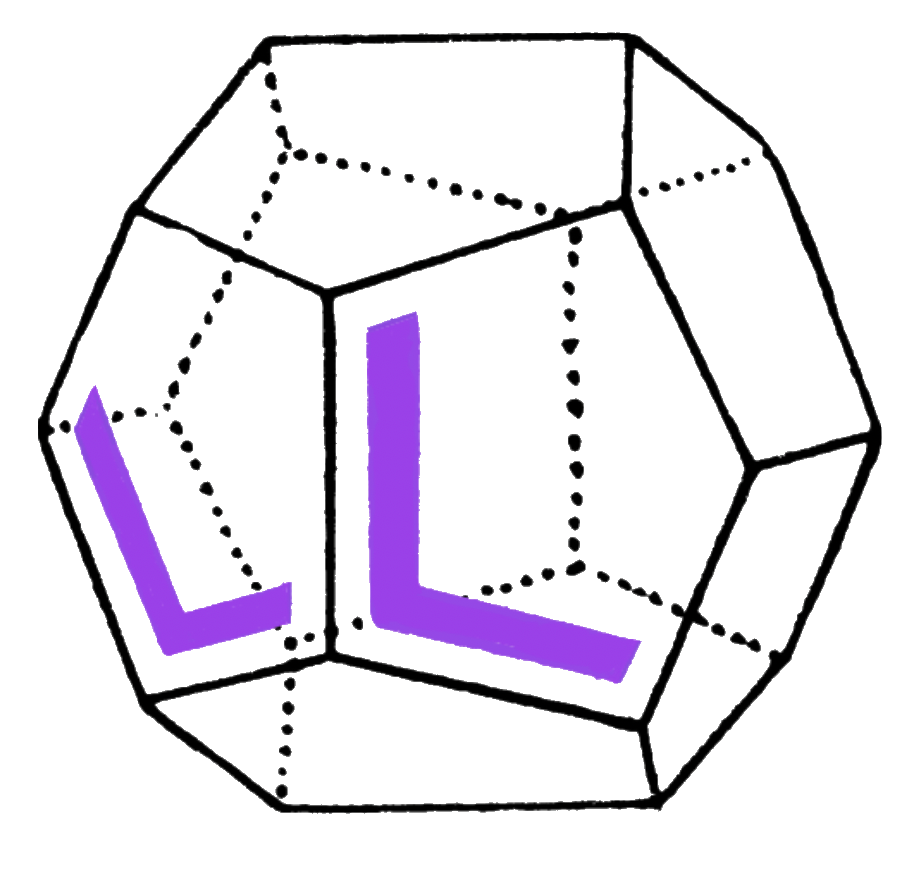
\includegraphics[width=2cm,height=2cm]{ll.png}}

    }}

\AddToShipoutPicture*
  {\put(470,767){
    \href{https://github.com/linlib/CategoriesandHilbertSpaces/StringDiagramGenerator.py}{\texttt{.py file}}
  }}

\AddToShipoutPicture*
  {\put(470,752){
    \href{https://github.com/linlib/ThreeWhiteheadTheoremsandThreePuppeSequences/ThreeWhiteheadTheoremsandThreePuppeSequences.tex}{\texttt{.tex file}}\\

  }}


\AddToShipoutPicture*
  {\put(470,737){

    \href{http://linearlibrary.net/ThreeWhiteheadTheoremsandThreePuppeSequences/ThreeWhiteheadTheoremsandThreePuppeSequences.pdf}{\texttt{.pdf file}}\\

  }}

  \AddToShipoutPicture*
  {\put(470,722){
    \href{https://github.com/linlib/ThreeWhiteheadTheoremsandThreePuppeSequences/ThreeWhiteheadTheoremsandThreePuppeSequences.lean}{\texttt{.lean file}}

  }}

\ \\

%LEAN: 
\begin{center}
\begin{tcolorbox}[width=5.8in,colback={white},coltitle=white]
\begin{center}
\ \\
\scalebox{3}{\texttt{∞-Spaces}}\\
\ \\
\end{center}
\end{tcolorbox}
\end{center}
\ \\
{\footnotesize
\begin{center}
\scalebox{1.1}{
\begin{tabular}{|| l | l || l | l | l  || l | l || l | l | l  || } 
\hline
$\texttt{Mon}$ & \texttt{D(}∞\texttt{-Cat)} & Σ⃗ & Ω⃗ & P⃗ & $\texttt{InfPreShf}$ & \texttt{D(}∞\texttt{-Cat/C)} & σ⃗ & ω⃗ & p⃗ \\
\hline
$\texttt{ComMon}$ & \texttt{D(}∞\texttt{-Grpd)} & Σ⃡ & Ω⃡ & P⃡  & $\texttt{IntAct}$ & \texttt{D(}∞\texttt{-Grpd/G)} & σ⃡ & ω⃡ & p⃡\\
 \hline
$\texttt{IntGrp}$ & \texttt{D(}∞\texttt{-Grpd₀)} & Σ & Ω & P  & $\texttt{IntAct₀}$ & \texttt{D(}∞\texttt{-Grpd₀/G₀)} & σ & ω & p \\
 \hline
\end{tabular}}
\end{center}}
\ \\
%LEAN: 
\begin{center}
\begin{tcolorbox}[width=6in,colback={white}]
\begin{center}
\ \\
\end{center}
\end{tcolorbox}
\end{center}

%LEAN: 
\begin{center}
\begin{tcolorbox}[width=4.13in,colback={white},coltitle=white]
\scalebox{1.5}{E. Dean Young}
\end{tcolorbox}
\end{center}


\begin{center}
\texttt{Plans to prove three variations of the}\\
\texttt{Whitehead theorem of homotopy groups in}\\
\texttt{Lean 4, with extensive use of Mathlib 4}
\end{center}


\thispagestyle{empty}


\newpage


\begin{center}

\pagecolor{white}
\color{black}




\end{center}

\thispagestyle{empty}




\newpage
\pagecolor{white}
\color{black}
\ \\
\ \\
\thispagestyle{empty}
\begin{center}
Copyright\ \textcopyright \ October 19th 2023 Elliot Dean Young and Jiazhen Xia.\ All rights reserved.\\
\end{center}
\large %%%%%%%% HERE IS THE large LARGE size textsize set text size
\newpage 
\ \\
\ \\
\ \\
\ \\
\ \\
\ \\
\ \\
\ \\
\ \\
\ \\
\ \\
\thispagestyle{empty}
 
\newpage

\ \\
\ \\
\ \\
\ \\
\ \\
\ \\
\ \\
\ \\
\ \\
\ \\
\ \\

We wish to acknowledge the collaborative efforts of E. Dean Young and Jiazhen Xia. Dean Young initially formulated the introduction with twelve goals, posting them on the Lean Zulip in August of 2023. Together the authors are pursuing these plans as a long term project.\\



\newpage



\newpage



\section{Introduction}

In this document I would like to develop a construction of the classifying space functor which can be applied indefinitely.\\

Segal ∞-Spaces and their relationship with 

explore derivations and connections.

In this section, which makes use of the previous section concerning Haar integral, I intend to cover the ordinary versions of Poincare duality, Pontrjagin duality, and Fourier duality, as well as versions of these theorems using language enabled by the previous repositories. This won't culminate until far into the future, so for now I have jotted down some sketches.\\


\section{Contents}


{
\footnotesize
\begin{longtable}{|| l || l ||} 
\hline
\multicolumn{1}{||c||}{$\texttt{Section}$} & \multicolumn{1}{|c||}{$\texttt{Description}$} \\
\hline
\hline
Unfinished & \\
\hline
Contents & \\
\hline
Unicode & \\
\hline
Introduction & \\
\hline \hline
\multicolumn{2}{||c||}{\texttt{PART I: } ABELIAN GROUPS AND ∞-SPACES} \\
\hline \hline
 \multicolumn{2}{||c||}{\texttt{Chapter 1: }Abelian Groups} \\
\hline \hline
 &  \\
\hline \hline
 \multicolumn{2}{||c||}{\texttt{Chapter 2: }Tensor Product of Abelian Groups} \\
\hline \hline
 &  \\
 \hline \hline
 \multicolumn{2}{||c||}{\texttt{Chapter 3: }Rings and Modules} \\
\hline \hline
 &  \\
 \hline \hline
 \multicolumn{2}{||c||}{\texttt{Chapter 4: }∞-Spaces} \\
\hline \hline
 &  \\
\hline \hline
\multicolumn{2}{||c||}{\texttt{Chapter 5: }Tensor Product of ∞-Spaces} \\
\hline \hline
 &  \\
 \hline \hline
  \multicolumn{2}{||c||}{\texttt{Chapter 6: }∞-Rings and ∞-Modules} \\
\hline \hline
 &  \\
 \hline \hline
 \multicolumn{2}{||c||}{\texttt{Chapter 7: }∞-Grpd ⇄ ∞-Space} \\
\hline \hline
 &  \\
\hline \hline
 \multicolumn{2}{||c||}{\texttt{Chapter 8: }Ring ⇄ ∞-Ring} \\
\hline \hline
 &  \\
\hline \hline
 \multicolumn{2}{||c||}{\texttt{Chapter 9: }Mod R ⇄ ∞-Mod R} \\
\hline \hline
 &  \\
\hline \hline
\multicolumn{2}{||c||}{\texttt{PART II: } DERIVATIONS AND CONNECTIONS} \\
\hline \hline
 &  \\
\hline \hline
\multicolumn{2}{||c||}{\texttt{Chapter 10: }Lie Algebras} \\
\hline \hline
 &  \\
\hline \hline
\multicolumn{2}{||c||}{\texttt{Chapter 11: }Lie Algebra Representations} \\
\hline \hline
 &  \\
\hline \hline
\multicolumn{2}{||c||}{\texttt{Chapter 12: }Derivations} \\
\hline \hline
 &  \\
\hline \hline
\multicolumn{2}{||c||}{\texttt{Chapter 13: }Connections} \\
\hline \hline
 &  \\
\hline \hline
\multicolumn{2}{||c||}{\texttt{Chapter 14: }L${}^{\infty}$-Algebras} \\
\hline \hline
 &  \\
\hline \hline
\multicolumn{2}{||c||}{\texttt{Chapter 15: }L${}^{\infty}$-Algebra Representations} \\
\hline \hline
 &  \\
\hline \hline
\multicolumn{2}{||c||}{\texttt{Chapter 16: }∞-Derivations} \\
\hline \hline
 &  \\
\hline \hline
\multicolumn{2}{||c||}{\texttt{Chapter 17: }∞-Connections} \\
\hline \hline
 &  \\
\hline \hline
\end{longtable}
}



\iffalse
https://redprl.org/
agda
rzk (new!)

Filippo A. E. Nuccio: Hi Dean, thanks for reaching out! I have had a brief look at your pdf and your lean code. Can you give some more details about your project, what you are exactly aiming at (integrating mathlib? writing a book on your own? writing a thesis to showcase your Lean expertise to apply for grad fellowship)? In particular, how can I provide feedback exactly?

Dean Young: Sorry for my late reply Filippo.

My collaborator (Jiazhen Xia) and I have a main goal of making a Mathlib PR. It would be helpful to get tips, points of importance, and suggestions for changes that would make it more likely to be accepted. We've set aside about a year to work through it, and we're taking the time to make as many changes as we need to ensure things like usability.

Separately, if you feel comfortable recommending me on this basis to PhD programs as well, it would improve the strength of my applications by a lot.

Dean Young: The most important kind of feed back is, what are some considerations in making the Whitehead theorem and Puppe sequence things that people would use? We are especially interested in this from the perspective of algebraic geometry.

Filippo A. E. Nuccio: Dear Dean, it is my turn to apologise for a late reply. I have seen your project and it is huge: I think that if you want to reasonably complete in a finite amount of time and to start doing PR's you should really identify a first much smaller goal.

Filippo A. E. Nuccio: I am not an expert in algebraic topology "in the modern sense", I would love to see the Whitehead theorem spelt down in purely topological terms, and this would certainly be a result in its own without the "need" for any application.

Filippo A. E. Nuccio: On the other hand, I see things that are already in mathlib, like pullback and pushouts: are you aware that you won't need to develop them?

Filippo A. E. Nuccio: The take-home message is really: start with a very small PR. Huge ones are hard to check, and if you got something wrong you'd rather discover it sooner than later.

Filippo A. E. Nuccio: If you want to continue the discussion, I would suggest that

You identify this small contribution, even if on the very long run you are aiming at Whitehead/Puppe
You discuss this small contribution in the public chat
You strive for it and try to make this first small PR. If it works, you'll make a second one. I was involved in LTE and one of the reasons it will be difficult to make a global PR is that it is too big and many things have diverged from themaster version of mathlib.
Filippo A. E. Nuccio: Concening your PhD, can I ask more details? Where are you based, where would you like to look for programs, have you a math/CS background, what is your primary scientific interest, how long is your NYU program?
\fi

\iffalse
https://mathoverflow.net/questions/464176/bⁿ-and-coherence
\fi


after this we develop chain complexes of these.\\


The table of contents below reflects the tentative long-term goals of the authors, with the main goal the pursuit of the Whitehead theorem for a point-set model involving Mathlib's predefined homotopy groups.\\

\begin{enumerate}
\item cup and cap product
\end{enumerate}

Ideas for future applications:

\begin{enumerate}
\item \url{https://arxiv.org/pdf/2206.13563.pdf}
\end{enumerate}

\begin{enumerate}
\item One of the basic things I wanted out of this was homotopy colimit preserving maps (Eⁱⁿᶠ-Alg A)ᵒᵖ ⭢ ∞-Grpd
\end{enumerate}


\part{PART I: ABELIAN GROUPS AND ∞-SPACES}

{
\footnotesize
\begin{center}
\begin{tabular}{||l || l || l || l ||} 
 \hline
  \multicolumn{4}{||c||}{\texttt{Eight Structures}} \\
 \hline
 \multicolumn{2}{||c||}{\texttt{Strict}}  &  \multicolumn{2}{||c||}{\texttt{Lax}} \\
 \hline
 \texttt{Unitial} &  \texttt{Actional}  &  \texttt{Unitial} &  \texttt{Actional}\\
 \hline \hline
 \texttt{InternalMonoid}  & \texttt{InternalMonoidAction} & \texttt{OperadicMonoid} & \texttt{OperadicMonoidAction} \\ 
 \hline
 \texttt{InternalCommutative Monoid} & \texttt{InternalCommutativeMonoidAction} & \texttt{OperadicMonoid} & \texttt{OperadicMonoidAction} \\ 
 \hline
 \hline
\end{tabular}
\end{center}
}


\chapter{Abelian Groups}

Abelian groups are internal groups in internal groups.



\chapter{Tensor Product of Abelian Groups}




\chapter{Rings and Modules}

make sure to include Alg




\chapter{∞-Spaces}

The little squares operad is 

\begin{center}
OperadicGroup • OperadicGroup  : ∞-Cat\_(A) ⭢ ∞-Cat\_(A) 
\end{center}

"Operadic groups in operadic groups" in O²

\begin{center}
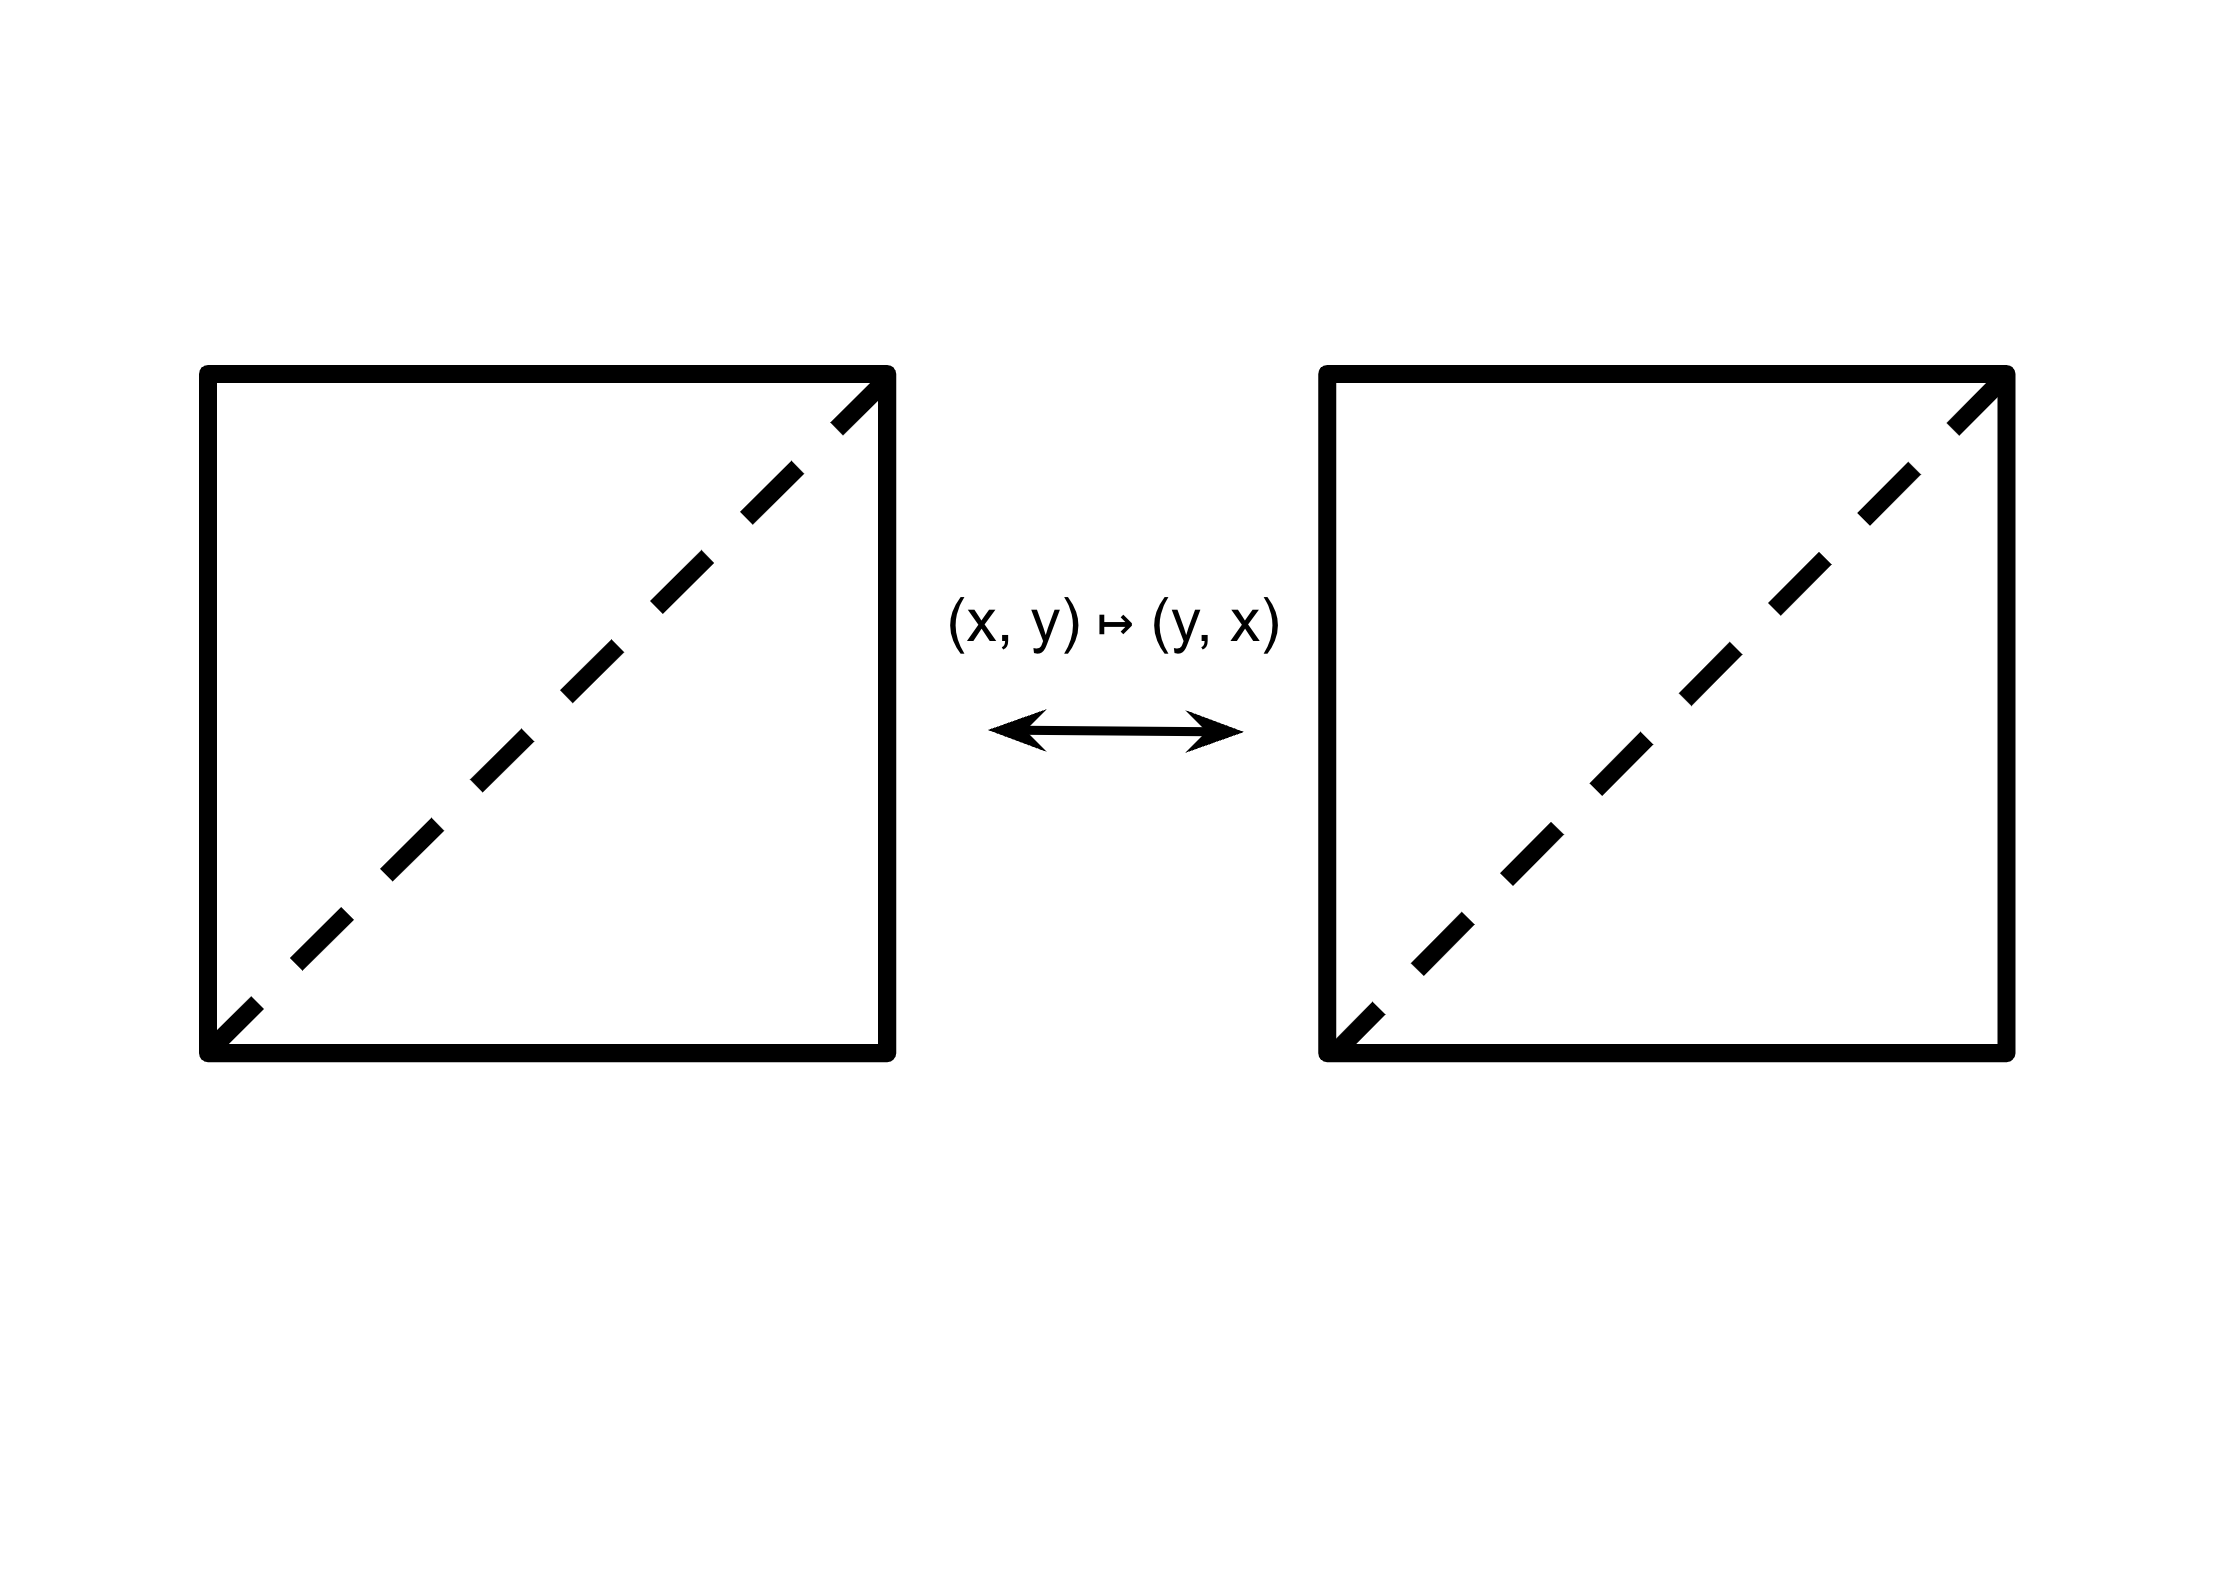
\includegraphics[width=7.5cm,height=5cm]{littlesquaresA.png}
\end{center}

\begin{center}
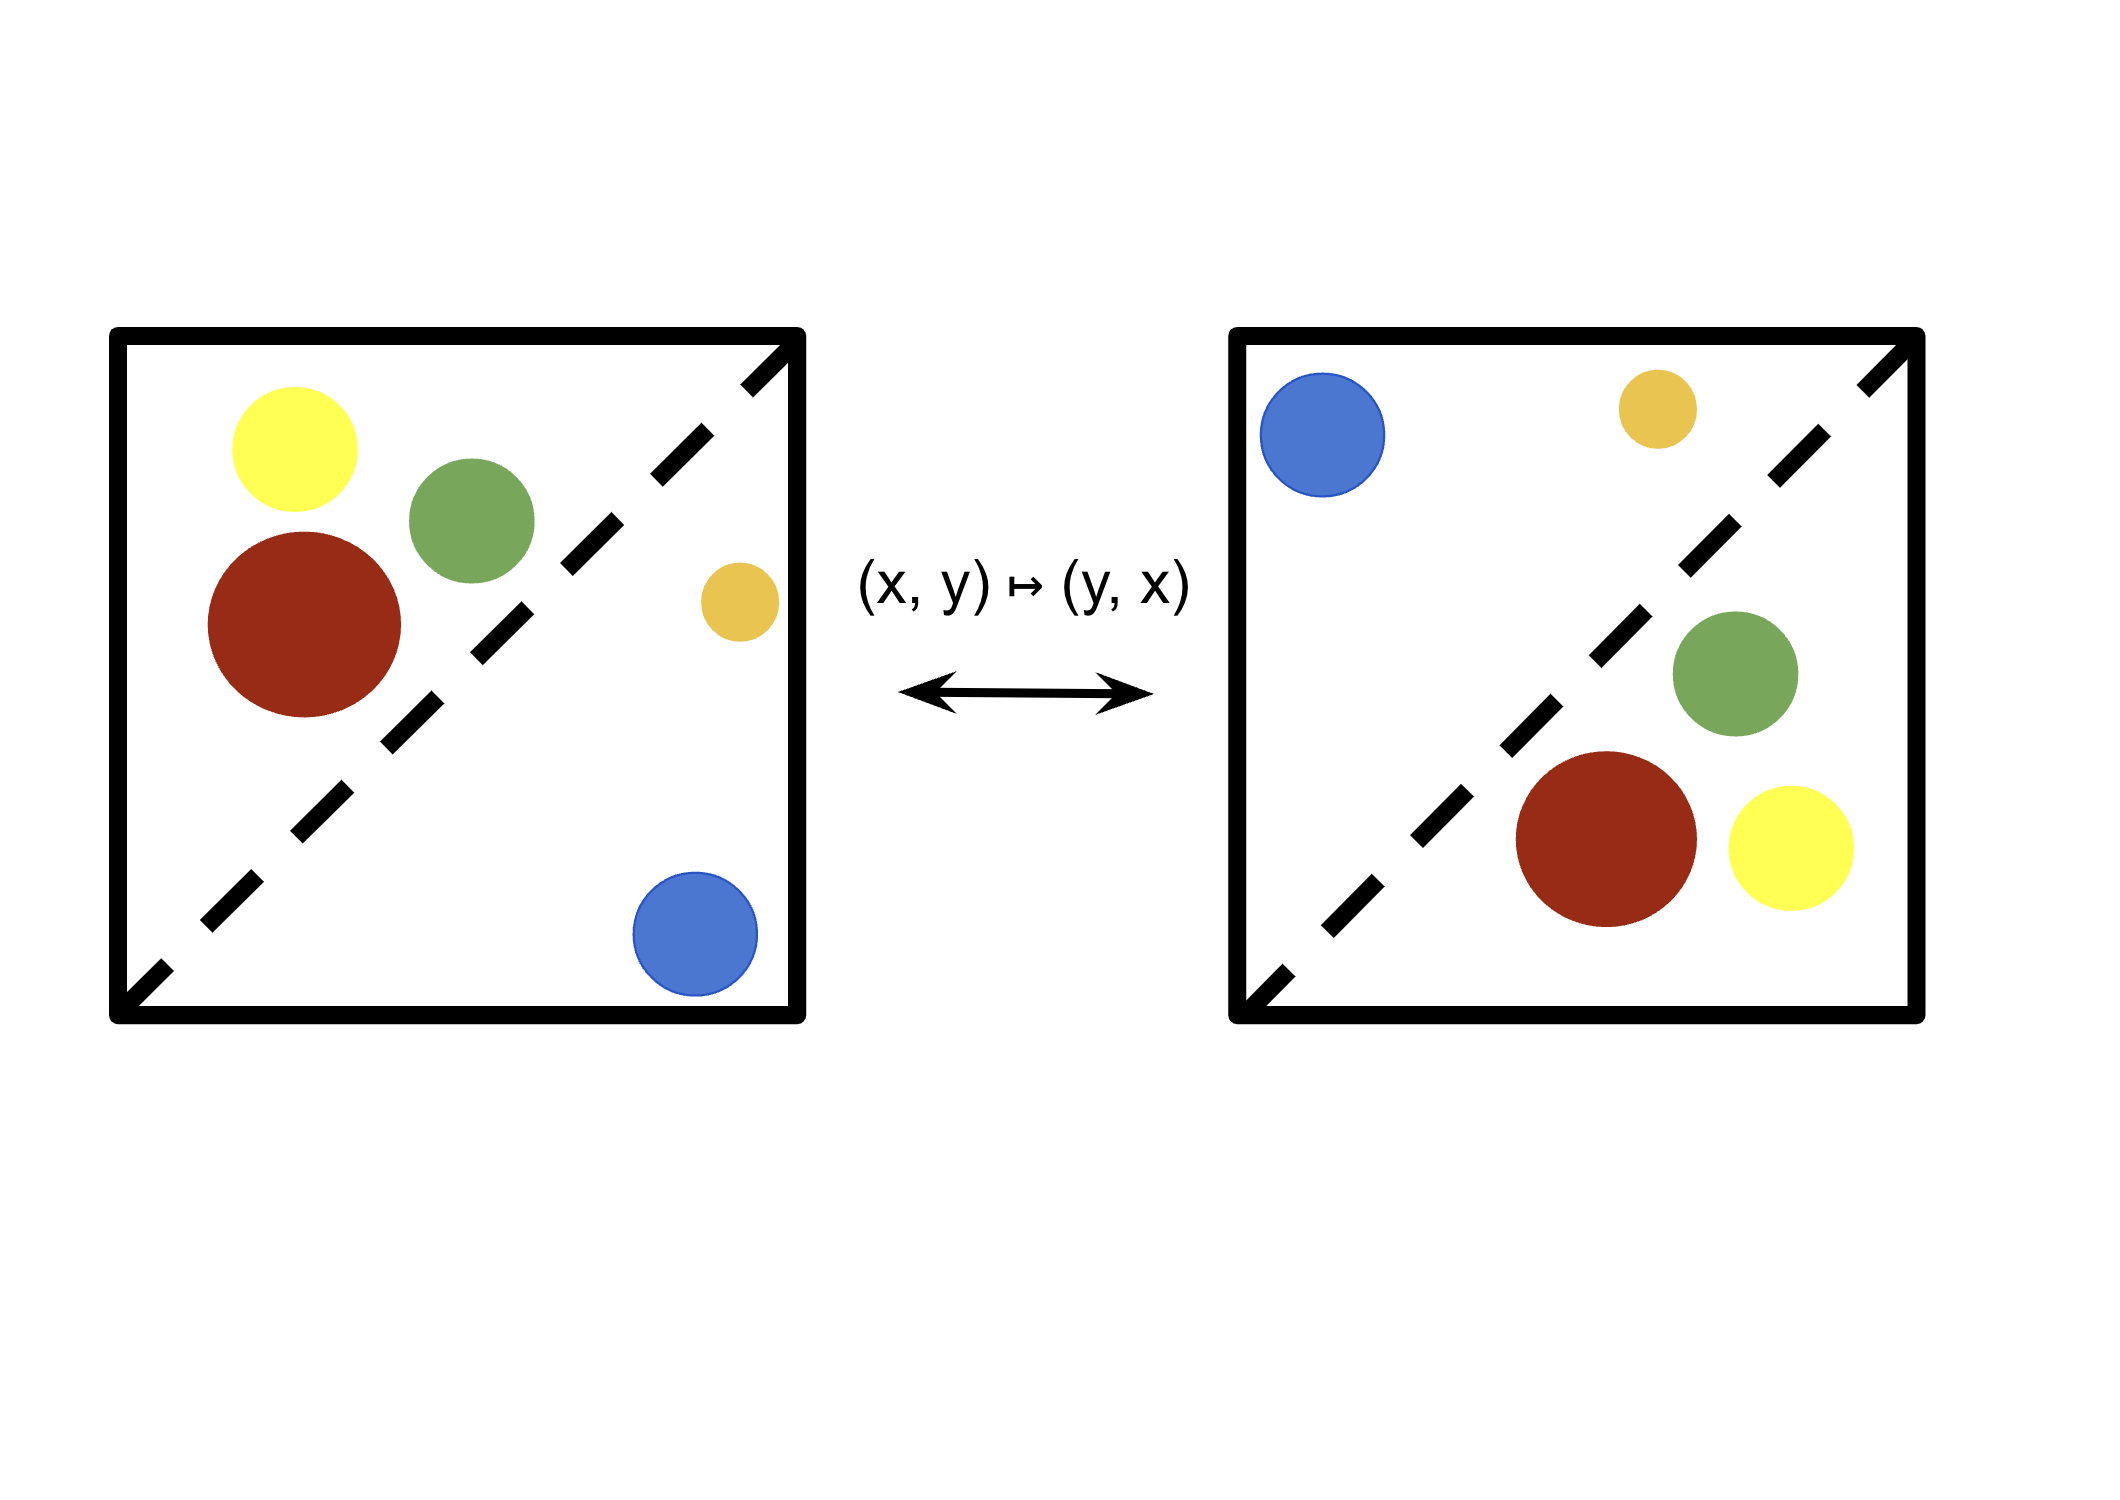
\includegraphics[width=7.5cm,height=5cm]{littlesquaresB.png}
\end{center}

The commutative nature of composition in the little squares operad is interesting.

\begin{center}
OperadicGroup² ∞\_(∞-Grpd)
\end{center}



\iffalse
In the repository concerning classifying spaces, I . 

In the repository

OperadicCategory² ∞-Cat, OperadicGroupoid² ∞-Grpd, and OperadicGroup² ∞-Grpd
\fi

OperadicGroup² : 

\begin{enumerate}
\item 
\end{enumerate}

Could ∞-spaces be operadic groups in operadic groups?

\iffalse
B¹.obj (M × N) ⭢ (B¹.obj M) × (B¹.obj N)

\fi

\iffalse
B¹.obj (M × N) ⭢ (B¹.obj M) × (B¹.obj N)
gives

"the little squares operad"
\fi

\iffalse
- Embedding Ringᵒᵖ              into ∞-presheaves in ∞-spaces
- Embedding DistributiveLattice into ∞-presheaves in ∞-spaces
- Embedding Scheme              into ∞-presheaves in ∞-spaces
\fi

\iffalse

https://leanprover.zulipchat.com/#narrow/stream/287929-mathlib4/topic/Definition.20of.20group.20scheme.3F

\fi



\newpage
\ \\




\chapter{Tensor Product of ∞-Spaces}




\chapter{∞-Rings and ∞-Modules}

\iffalse
Besides that my ∞-spaces are different, I would like to make my Ainfinity and Einfinity objects as similar as possible.
\fi


make sure to include ∞-Alg...



\iffalse
- Embedding Ringᵒᵖ              into ∞-presheaves in ∞-spaces
- Embedding DistributiveLattice into ∞-presheaves in ∞-spaces
- Embedding Scheme              into ∞-presheaves in ∞-spaces
\fi

\iffalse
https://leanprover.zulipchat.com/#narrow/stream/116395-maths/topic/Ext.20and.20Tor
\fi





\chapter{∞-Grpd ⇄ ∞-Space}

{
\footnotesize
\begin{center}
\begin{tabular}{||l ||} 
 \hline
 \hline
Set ⇄ AbelianGroup \\
 \hline
∞-Grpd ⇄ ∞-Space \\
 \hline 
 \hline
Ring ⇄ ∞-Ring \\
 \hline
Mod R ⇄ ∞-Mod R \\
 \hline
 \hline
\end{tabular}
\end{center}
}

\begin{enumerate}
\item πₙ of an ∞-space arising from an ∞-groupoid vs. Hₙ ...
\item 
\item \iffalse https://leanprover.zulipchat.com/#narrow/stream/116395-maths/topic/homology \fi
\item 
\end{enumerate}


\chapter{Ring ⇄ ∞-Ring}

\iffalse
Λ*... use a subscript with round braces for the strict and lax variations
Ω as well
λ for actional
ω for actional
\fi


\chapter{Mod R ⇄ ∞-Mod R}

\iffalse
Λ*... use a subscript with round braces for the strict and lax variations
Ω as well
λ for actional
ω for actional
\fi



\part{PART II: DERIVATIONS AND CONNECTIONS}

{
\footnotesize
\begin{center}
\begin{tabular}{|| l || l ||} 
\hline
(Alg R)/B ⇄ Mod B  & (∞-Alg R)/B ⇄ ∞-Mod B \\
 \hline 
??? ⇄ ???  & ??? ⇄ ??? \\
 \hline
\end{tabular}
\end{center}
}

\iffalse
https://en.wikipedia.org/wiki/Connection_(vector_bundle)
\fi




\chapter{Lie Algebras}




\chapter{Lie Algebra Representations}





\chapter{Derivations}

\begin{enumerate}
\item I would like to first construct the lie-algebra of derivations using the spectrum \texttt{Ωⁱⁿᶠ.obj X}. It seems related to coalgebra endomorphisms from \texttt{Ωⁱⁿᶠ.obj X} to itself.\\
\item Lie algebras and Derₖ(A,A)
\end{enumerate}


\chapter{Connections}

\begin{enumerate}
\item I would like to first construct the lie-algebra representation of flat connections using the spectrum \texttt{ωⁱⁿᶠ.obj X).obj V}.
\item \iffalse https://en.wikipedia.org/wiki/Connection_(vector_bundle)\fi
\item Lie algebra representations and ...
\item 
\item 
\item \iffalse https://en.wikipedia.org/wiki/Connection_(vector_bundle)\fi
\item Somehow connections are the dual of the free abelian group action
\end{enumerate}

\iffalse We can define differentiable and connective functionals in this context as well. \fi

\iffalse
https://en.wikipedia.org/wiki/Connection_form
\fi





    \iffalse
    https://amathew.wordpress.com/2011/05/14/the-cotangent-complex-i-group-objects-in-categories-of-algebras/
    \fi



    \iffalse
    I loaded them up onto degree negative one.
    \fi



    Some goals:
    \begin{enumerate}
    \item 
    \end{enumerate}

    \begin{enumerate}
    \item smooth (etale locally ???)
    \item analytic (etale locally ???)
    \item [ℂP¹,ℂP¹] ≅ ℂ(x)
    \item Our ℝ is ∂.obj ℤ regarded as an object in [γ⃗,∞\_(∞-Grpd)]
    \item B.obj det : B.obj U(n) ⭢ B.obj U(1)
    \item Which E${}_{\infty}$ Space have a Chern class?
    \end{enumerate}

    Cohomology with coefficients in $\texttt{[-,Bℂˣ]}$ plays a .\\

    \iffalse
    https://www.universiteitleiden.nl/binaries/content/assets/science/mi/scripties/bachbecker.pdf
    \fi

\begin{enumerate}
\item \iffalse https://en.wikipedia.org/wiki/Connection_(vector_bundle) \fi
\item d2 is wedge with (representable...)
\end{enumerate}



\chapter{L${}^{\infty}$ Algebras}




\chapter{L${}^{\infty}$ Algebra Representations}





\chapter{∞-Derivations}




\chapter{∞-Connections}





\iffalse

{
\footnotesize
\begin{longtable}{|| l || l ||} 
\hline
\multicolumn{1}{||c||}{$\texttt{Section}$} & \multicolumn{1}{|c||}{$\texttt{Description}$} \\
\hline \hline
 &  \\
\hline \hline
 &  \\
\hline \hline
\end{longtable}
}


\multicolumn{2}{||c||}{\texttt{Chapter 18: }Kan Extensions} \\
\hline
??? & ???\\
\hline \hline 
\multicolumn{2}{||c||}{\texttt{Chapter 19: }Isbell Duality} \\
\hline
??? & ???\\
\hline \hline 
\multicolumn{2}{||c||}{\texttt{Chapter 20: }Adjoints} \\
\hline
??? & ???\\
\hline \hline 
\multicolumn{2}{||c||}{\texttt{Chapter 18: }Pointed Kan Extensions} \\
\hline
??? & ???\\
\hline \hline


\fi




\iffalse
{
\footnotesize
\begin{center}
\begin{tabular}{||l || l || l || l ||} 
 \hline
  \multicolumn{4}{||c||}{\texttt{Twelve Structures}} \\
 \hline
 \multicolumn{2}{||c||}{\texttt{Strict}}  &  \multicolumn{2}{||c||}{\texttt{Lax}} \\
 \hline
 \texttt{Unitial} &  \texttt{Actional}  &  \texttt{Unitial} &  \texttt{Actional}\\
 \hline \hline
 \texttt{InternalCategory}  & \texttt{InternalPresheaf} & \texttt{OperadicCategory} & \texttt{OperadicPresheaf} \\ 
 \hline
 \texttt{InternalGroupoid} & \texttt{InternalGroupoidAction} & \texttt{OperadicGroupoid} & \texttt{OperadicGroupoidAction} \\ 
 \hline
\texttt{InternalGroup} & \texttt{InternalGroupAction} & \texttt{OperadicGroup} & \texttt{OperadicGroupAction} \\ 
 \hline 
\end{tabular}
\end{center}
}
\fi


\iffalse 
χ⃗ : ??? ∞\_(∞-Grpd₀)/X₀ ⭢ ∞\_(∞-Grpd₀)/Y₀ 
\fi 

In this repository, I would like to think about the relationship between homotopy colimits, directed homotopy colimits, and homotopy colimits over based connected ∞-groupoids and one object ∞-groupoids, pariticularly as it concerns the six ``fibrant replace and forget" functors.\\

I would also like to incorporate two notions of the formal addition of an interval object and directed interval object, as well as six theorems concerning monadicity that are related to it.\\

\iffalse
It could make sense to define a geometric map here
\fi







\iffalse
\begin{center}
% https://tikzcd.yichuanshen.de/#N4Igdg9gJgpgziAXAbVABwnAlgFyxMJZABgBpiBdUkANwEMAbAVxiRAB12cYAPHf4MgDCgJVxAarilAeEScA+gApJAWiF0cASgoBfEJtLpMufIRRkAjFVqMWbae3lLO3PgJXrAIgRDtu-djwEiAMzkFvTMrIggyAAi4lKyjrz8OMAKyqoaXnogGL5GgaTm1KHWEbb2Cc7JaeqabhVJwFFeFjBQAObwRKAAZgBOEAC2SGQgOBBIptQARjBgUEgBI8XhIHKA48CA9BuAKTtqAHQQUwBWAARCOll9gxPUY8PTs-OIi0VWK+uAjpB7Bydn3iCXQyeN3GiEmljCbHqAjkgEngQDrBLsABaDY4AMTUmm2IGoDDoMwYAAUDH5jCAGDBujhsSAZnMFsQ-gC7qMQQAmF4QiJQ5JyGAI5EDNEY97U2mPRaM-qA9ks5nLSFcRLQvlIlHozQiyVXUHAhYckocRWVFLw1WC9Wai5SpAy25A8EG9bbL5HY5RUUPelawFBWWIGVi+n6t5rT77V3uzRaIA
\begin{tikzcd}
{\texttt{[Cᵒᵖ,∞\_(∞-Cat)]}} \arrow[d, "(χ𛲔).obj C", bend left] \arrow[rrr, "\texttt{(e⃗.hom F)}ॱ", bend left] &  &  & {[Dᵒᵖ,∞\_\texttt{(∞-Cat)]}} \arrow[lll, "\texttt{(e⃗.hom F)}ॱ"] \arrow[d, "(χ𛲔).obj D", bend left]               \\
∞\_(∞-\texttt{Cat)⁄C} \arrow[u, "(χॱ).obj C", bend left] \arrow[rrr, "\texttt{(ω⃗.hom F)}ॱ"]                   &  &  & ∞\_(∞\texttt{-Cat)}⁄\texttt{D} \arrow[lll, "\texttt{(ω⃗.hom F)}𛲔", bend left] \arrow[u, "(χॱ).obj D", bend left]
\end{tikzcd}
\end{center}
\fi


\iffalse

 the left adjoint to precomposition in the case of the derived completion functors:

\begin{enumerate}
\item (completion of an ∞-category with respect to the directed derived category D(∞-Cat))
\begin{center}
 χ⃗  : (X : ∞-Cat) → (Y : ∞-Cat) → ∞-Cat.hom X Y → Adjunction D([-ᵒᵖ,∞-Cat]) D([-ᵒᵖ,∞-Cat] )
\end{center}
\item (completion of an ∞-groupoid with respect to the directed derived category D(∞-Grpd)) χ⃡ : [-ᵒᵖ,D(∞-Grpd)] ⇄ [-ᵒᵖ,D(∞-Grpd)]
\begin{center}
 χ⃡ : (X : ∞-Grpd) → (Y :∞-Grpd) → ∞-Grpd.hom X Y → Adjunction [-ᵒᵖ,D(∞-Grpd)] [-ᵒᵖ,D(∞-Grpd)]
\end{center}
\item (completion of a based connected ∞-groupoid with respect to the category of based connected ∞-groupoids) χ : [-ᵒᵖ,D(∞-Grpd₀)] ⇄ [-ᵒᵖ,D(∞-Grpd₀)] :
\begin{center}
 χ : (X : ∞-Grpd₀) → (Y :∞-Grpd₀) → ∞-Grpd₀.hom X Y → Adjunction [-ᵒᵖ,D(∞-Grpd₀)] [-ᵒᵖ,D(∞-Grpd₀)]
\end{center}
\end{enumerate}



\begin{enumerate}
\item E, e and the various `up to homotopy' structures (six)
\item 
\end{enumerate}




I like to use a notation of upper and lower dots for the left and right adjoint in $\texttt{Lean 4}$, but it requires specific fonts that not all systems have, and the two different characters do not always display like one another.\\

These three functors produce 

\begin{enumerate}
\item Links back to the category section concerning the category of elements and how it can be used to express pointed Kan extensions.
\item χॱ.hom : Functor D(∞-Cat) ⇄ D(∞-Cat) : χ𛲔
\item χ
\item \iffalse ∞_(∞-Lan) : D(∞-Cat) ⭢ \fi
\end{enumerate}

After establishing several interesting features of Lan D(∞-Cat),  Fᵒᵖ : [Cᵒᵖ,D(∞-Cat)] ↔ [Dᵒᵖ,D(∞-Cat)] : Cmp



[D(∞-Grpd), D(∞-Grpd₀)]

Some further goals:
\begin{enumerate}
\item Connecting the dots with various Mathlib 4 structures:
\begin{enumerate}
\item Projective space over an algebraically closed field as an ∞-topos
\item The Segre embedding as a map of ∞-topoi
\item Embedding various common categories into ∞-topoi
\item 
\end{enumerate}
\end{enumerate}

\section{Lan D(∞-Cat)}


\iffalse

[-,∞-Cat]
[-,∞-Grpd]
[-,∞-Grpd₀]


[-,∞-Cat]
[-,∞-Grpd]
[-,∞-Grpd₀]

\fi


\chapter{ETCC Signature 3}

ETCC signature 3 says that 

\begin{enumerate}
\item D(∞\_(∞-Cat)) classifies D(∞\_(∞-Cat)⁄-) : ∞\_(∞-Cat) ⭢ ∞\_(∞-Cat)
\item 
\end{enumerate}

\iffalse
\begin{definition}
The separable closure
\end{definition}

\begin{definition}
The maximal unramified extension
\end{definition}

\begin{definition}
The (abelian) separable closure
\end{definition}

\begin{definition}
The (abelian) maximal unramified extension
\end{definition} 
\fi



\iffalse

  \chapter{Chapter 2: Pullback Systems} \\\
\\\
\section{$\texttt{pullback\_systems}$}
$\texttt{pullback\_systems}$ is a type defined in this kernel to handle derived directed homotopy pullback and directed homotopy pullback of something with itself (which we take to be directed path space [Δ1,-]). It also stores the information of the category D(∞-Cat), as well as D(∞-Cat⁄C) for each C : D(∞-Cat). D(∞-Cat) has a universe object ∞ as well, and a point *, and a map ⊥ : * → ∞. Various constructions associated to ∞-categories with a kind of universe object form the only example of a pullback system that we will use here, and yet it may prove to be useful in understanding how to force a situation in which the Whitehead theorem applies later on. \\
%LEAN: defining a pullback system
\begin{center} \begin{tcolorbox}[width=5in,colback={white},title={\begin{center}\texttt{Lean \thelcounter} \addtocounter{lcounter}{1} \end{center}},colbacktitle=Blue,coltitle=black] \begin{minted}[breaklines, escapeinside=||]{lean}

 /-
structure pullback_system where
Obj : Cat
Pnt : Obj
CmpObj : Obj.Obj → Cat CmpHom : (C : Obj.Obj) →
(D : Obj.Obj) →
(F : Obj.Hom C D) → (Functor (CmpObj C) (CmpObj D)) -- note this may need tweaking, but it should produce a functor F : D(∞-Cat/D) → D(∞-Cat/C) for each
--
CmpIdn : (C : Obj.Obj) → ((CmpHom C C (𝟙_(Obj) C)) = 𝟏_(𝐂𝐚𝐭) (CmpObj C)) CmpCmp : (C : Obj.Obj) → (D : Obj.Obj) → (E : Obj.Obj) → (F : Obj.Hom C D) → (G :
Obj.Hom D E) → (((CmpHom D E G) •_(𝐂𝐚𝐭) (CmpHom C D F)) = CmpHom C E (G ∘_(Obj) F))
Fix : Obj ≃_(𝐂𝐚𝐭) (CmpObj Pnt) Pul : (C : Obj.Obj) →
(D : Obj.Obj) →
(F : Obj.Hom C D) →
(𝐂𝐚𝐭.Hom (CmpObj D) (CmpObj C)).Obj
η : (C : Obj.Obj) → (D : Obj.Obj) → (F : Obj.Hom C D) → ((𝐂𝐚𝐭.Hom (CmpObj C) (CmpObj C)).Hom (𝟏_(𝐂𝐚𝐭) (CmpObj C)) ((Pul C D F) •_(𝐂𝐚𝐭) (CmpHom C D F)))
ε : (C : Obj.Obj) → (D : Obj.Obj) → (F : Obj.Hom C D) → ((𝐂𝐚𝐭.Hom (CmpObj D) (CmpObj D)).Hom ((CmpHom C D F) •_(𝐂𝐚𝐭) (Pul C D F)) (𝟏_(𝐂𝐚𝐭) (CmpObj D)))
Id1 : (C : Obj.Obj) → (D : Obj.Obj) → (F : Obj.Hom C D) → (AdjId1 𝐂𝐚𝐭 (CmpObj C) (CmpObj D) (CmpHom C D F) (Pul C D F) (η C D F) (ε C D F))
Id2 : (C : Obj.Obj) → (D : Obj.Obj) → (F : Obj.Hom C D) → (AdjId2 𝐂𝐚𝐭 (CmpObj C) (CmpObj D) (CmpHom C D F) (Pul C D F) (η C D F) (ε C D F))
Inf : Obj.Obj
Ovr : Obj.Hom Pnt Inf
Chi : (C : Obj.Obj) → (F : (CmpObj C).Obj) → ((Obj.Hom) C Inf)
-- ??? : (C : Obj.Obj) → (F : (Cmp C).Obj) → ((Pul C Inf (χ C f)).Hom Pnt Inf Ovr = f) -/
\end{minted} \end{tcolorbox} \end{center}
The last axiom above is a bit tricky, but it is related to straightening and unstraightening.\\ We use the notation like this:
%LEAN:

 \begin{center} \begin{tcolorbox}[width=5in,colback={white},title={\begin{center}\texttt{Lean \thelcounter} \addtocounter{lcounter}{1} \end{center}},colbacktitle=Blue,coltitle=black] \begin{minted}[breaklines, escapeinside=||]{lean}
notation "D(" Γ "⁄-)" => "Γ"
\end{minted} \end{tcolorbox} \end{center}
In the remainder of this section, I made some boxes which altogether filled out make pullback systems into a category.\\
%LEAN: defining a map of pullback systems
\begin{center} \begin{tcolorbox}[width=5in,colback={white},title={\begin{center}\texttt{Lean \thelcounter} \addtocounter{lcounter}{1} \end{center}},colbacktitle=Blue,coltitle=black] \begin{minted}[breaklines, escapeinside=||]{lean}
-- defining a map of pullback systems
structure PulHom (Γ1 : pullback_system) (Γ2 : pullback_system) where
Obj : (𝐂𝐚𝐭.Hom Γ1.Obj Γ2.Obj).Obj
Obj2 : (C : Γ1.Obj.Obj) → (𝐂𝐚𝐭.Hom (Γ1.CmpObj C) (Γ2.CmpObj (Obj.Obj C))).Obj -- plays well with CmpHom?
-- Idn
-- Cmp
\end{minted} \end{tcolorbox} \end{center}
%LEAN: defining the identity map of two pullback systems
\begin{center} \begin{tcolorbox}[width=5in,colback={white},title={\begin{center}\texttt{Lean \thelcounter} \addtocounter{lcounter}{1} \end{center}},colbacktitle=Blue,coltitle=black] \begin{minted}[breaklines, escapeinside=||]{lean}
-- defining the identity map of two pullback systems def PulIdn (X : pullback_system) : PulHom X X := sorry
\end{minted} \end{tcolorbox}

 \end{center}
%LEAN: defining the composition of two pullback systems
\begin{center} \begin{tcolorbox}[width=5in,colback={white},title={\begin{center}\texttt{Lean \thelcounter} \addtocounter{lcounter}{1} \end{center}},colbacktitle=Blue,coltitle=black] \begin{minted}[breaklines, escapeinside=||]{lean}
-- defining the composition of two pullback systems
def PulCmp (X : pullback_system) (Y : pullback_system) (Z : pullback_system) (_ : PulHom X Y) (_ : PulHom Y Z) : PulHom X Z := sorry
\end{minted} \end{tcolorbox} \end{center}
%LEAN: proving the first identity law for maps of pullback systems
\begin{center} \begin{tcolorbox}[width=5in,colback={white},title={\begin{center}\texttt{Lean \thelcounter} \addtocounter{lcounter}{1} \end{center}},colbacktitle=Blue,coltitle=black] \begin{minted}[breaklines, escapeinside=||]{lean}
-- proving the first identity law for maps of pullback systems
def PulId1 (X : pullback_system) (Y : pullback_system) (f : PulHom X Y) : PulCmp X Y Y f (PulIdn Y) = f := sorry
\end{minted} \end{tcolorbox} \end{center}
%LEAN: proving the second identity law for maps of pullback systems
\begin{center} \begin{tcolorbox}[width=5in,colback={white},title={\begin{center}\texttt{Lean \thelcounter} \addtocounter{lcounter}{1} \end{center}},colbacktitle=Blue,coltitle=black] \begin{minted}[breaklines, escapeinside=||]{lean}
-- proving the first identity law for maps of pullback systems
def PulId2 (X : pullback_system) (Y : pullback_system) (f : PulHom X Y) : PulCmp X X Y (PulIdn X) f = f := sorry
\end{minted}

 \end{tcolorbox} \end{center}
%LEAN: proving the associativity law for maps of pullback systems
\begin{center} \begin{tcolorbox}[width=5in,colback={white},title={\begin{center}\texttt{Lean \thelcounter} \addtocounter{lcounter}{1} \end{center}},colbacktitle=Blue,coltitle=black] \begin{minted}[breaklines, escapeinside=||]{lean}
def PulAss (W : pullback_system) (X : pullback_system) (Y : pullback_system) (Z : pullback_system) (f : PulHom W X) (g : PulHom X Y) (h : PulHom Y Z) : PulCmp W X Z f (PulCmp X Y Z g h) = PulCmp W Y Z (PulCmp W X Y f g) h := sorry
\end{minted} \end{tcolorbox} \end{center}
%LEAN: constructing the category Pul of pullback systems
\begin{center} \begin{tcolorbox}[width=5in,colback={white},title={\begin{center}\texttt{Lean \thelcounter} \addtocounter{lcounter}{1} \end{center}},colbacktitle=Blue,coltitle=black] \begin{minted}[breaklines, escapeinside=||]{lean}
-- constructing the category Pul of pullback systems
def Pul : category := {Obj := pullback_system, Hom := PulHom, Idn := PulIdn, Cmp := PulCmp, Id1 := PulId1, Id2 := PulId2, Ass := PulAss}
notation "Loc" => Pul
\end{minted} \end{tcolorbox} \end{center}
\section{The Pullback System of Infinity Categories}
The pullback system will be able to encapsulate information associated to ∞-Cat, D(∞-Cat),
and D(∞-Cat⁄C), namely the derived directed homotopy pullback functor and its adjoint D(ω𛲔.hom f), derived postcomposition D(ωॱ.hom f).\\
$D(Γ)$ is the ``Obj" component from the above structure: %LEAN:

 \begin{center} \begin{tcolorbox}[width=5in,colback={white},title={\begin{center}\texttt{Lean \thelcounter} \addtocounter{lcounter}{1} \end{center}},colbacktitle=Blue,coltitle=black] \begin{minted}[breaklines, escapeinside=||]{lean}
def D (Γ : pulback_system) := Γ.Obj
\end{minted} \end{tcolorbox} \end{center}
Meanwhile, the categories $D($∞$-Cat⁄C)$ are formed from the the $\texttt{CmpObj}$ components in the above like this:
%LEAN:
\begin{center} \begin{tcolorbox}[width=5in,colback={white},title={\begin{center}\texttt{Lean \thelcounter} \addtocounter{lcounter}{1} \end{center}},colbacktitle=Blue,coltitle=black] \begin{minted}[breaklines, escapeinside=||]{lean}
def derived_category (Γ : pullback_system) (C : Γ.Obj.Obj) : 𝐂𝐚𝐭.Obj := Γ.CmpObj C
\end{minted} \end{tcolorbox} \end{center}
%LEAN:
\begin{center} \begin{tcolorbox}[width=5in,colback={white},title={\begin{center}\texttt{Lean \thelcounter} \addtocounter{lcounter}{1} \end{center}},colbacktitle=Blue,coltitle=black] \begin{minted}[breaklines, escapeinside=||]{lean}
-- notation "Cmp_(" Γ ")" => derived_category Γ notation "D(" Γ "⁄" C ")" => derived_category Γ C
\end{minted} \end{tcolorbox} \end{center}
\section{$\texttt{ω⃗\_(Γ) f}$}

 Each pullback system features a construction ω⃗ which is the directed homotopy pullback in the case of ∞-categories.\\
%LEAN: assembling the adjunction ω⃗_(Γ)
\begin{center} \begin{tcolorbox}[width=5in,colback={white},title={\begin{center}\texttt{Lean \thelcounter} \addtocounter{lcounter}{1} \end{center}},colbacktitle=Blue,coltitle=black] \begin{minted}[breaklines, escapeinside=||]{lean}
def directed_homotopy_pullback (Γ : pullback_system) (E : Γ.Obj.Obj) (B : Γ.Obj.Obj) (f : Γ.Obj.Hom E B) : (adjunction 𝐂𝐚𝐭) := sorry
\end{minted} \end{tcolorbox} \end{center}
%LEAN: notation for ω⃗_(Γ)
\begin{center} \begin{tcolorbox}[width=5in,colback={white},title={\begin{center}\texttt{Lean \thelcounter} \addtocounter{lcounter}{1} \end{center}},colbacktitle=Blue,coltitle=black] \begin{minted}[breaklines, escapeinside=||]{lean}
notation : 4000 "ω⃗_(" Γ ")" => pullback Γ
\end{minted} \end{tcolorbox} \end{center}
%LEAN: (ω⃗_(Γ) 𝟙_(?) C)𛲔 = 𝟏_(?) (ω⃗_(Γ) C)𛲔
\begin{center} \begin{tcolorbox}[width=5in,colback={white},title={\begin{center}\texttt{Lean \thelcounter} \addtocounter{lcounter}{1} \end{center}},colbacktitle=Blue,coltitle=black] \begin{minted}[breaklines, escapeinside=||]{lean}
--
/-
def pIdn : -/
\end{minted} \end{tcolorbox} \end{center}

 %LEAN: (ω⃗_(Γ) f)𛲔 •_(?) (ω⃗_(Γ) g)𛲔 = (p_(Γ) f ∘_(?) g)𛲔
\begin{center} \begin{tcolorbox}[width=5in,colback={white},title={\begin{center}\texttt{Lean \thelcounter} \addtocounter{lcounter}{1} \end{center}},colbacktitle=Blue,coltitle=black] \begin{minted}[breaklines, escapeinside=||]{lean}
--
/-
def pCmp : -/
\end{minted} \end{tcolorbox} \end{center}
\section{$\texttt{*\_(Γ)}$}
The terminal object is the $\texttt{Pnt}$ component, and will be pretty easy to fill out in our
upcoming semantics:
%LEAN:
\begin{center} \begin{tcolorbox}[width=5in,colback={white},title={\begin{center}\texttt{Lean \thelcounter} \addtocounter{lcounter}{1} \end{center}},colbacktitle=Blue,coltitle=black] \begin{minted}[breaklines, escapeinside=||]{lean}
-- def terminal_object (Γ : pullback_system) : Γ.Obj.α := Γ.Pnt
\end{minted} \end{tcolorbox} \end{center}
%LEAN:
\begin{center} \begin{tcolorbox}[width=5in,colback={white},title={\begin{center}\texttt{Lean \thelcounter} \addtocounter{lcounter}{1} \end{center}},colbacktitle=Green,coltitle=black] \begin{minted}[breaklines, escapeinside=||]{lean}
notation : 3000 "*_(" Γ ")" => terminal_object Γ
\end{minted} \end{tcolorbox}

 \end{center} \section{$\texttt{∞\_(Γ)}$}
The $\texttt{Inf}$ component is the internal universe in D(∞-Cat). I didn't mention this before since it's really tricky to get right in a way which doesn't encumber the approach.\\
%LEAN:
\begin{center} \begin{tcolorbox}[width=5in,colback={white},title={\begin{center}\texttt{Lean \thelcounter} \addtocounter{lcounter}{1} \end{center}},colbacktitle=Blue,coltitle=black] \begin{minted}[breaklines, escapeinside=||]{lean}
def universe_object (Γ : pulback_system) : Γ.Obj.Obj := Γ.Inf
\end{minted} \end{tcolorbox} \end{center}
%LEAN:
\begin{center} \begin{tcolorbox}[width=5in,colback={white},title={\begin{center}\texttt{Lean \thelcounter} \addtocounter{lcounter}{1} \end{center}},colbacktitle=Blue,coltitle=black] \begin{minted}[breaklines, escapeinside=||]{lean}
notation "∞_(" Γ ")" => universe_object Γ
\end{minted} \end{tcolorbox} \end{center}
\section{$\texttt{⊥\_(Γ)}$}
Here we define the "false" map, which consists of a point mapping into the universe object. Directed homotopy pullback of F : C → ∞\_(Γ) is of very special significance, and related to Lurie's ``straightening" and ``unstraightening".\\
%LEAN: defining ⊥_(Γ) : Γ.Obj.Hom *_(Γ) ∞_(Γ)
\begin{center} \begin{tcolorbox}[width=5in,colback={white},title={\begin{center}\texttt{Lean \thelcounter} \addtocounter{lcounter}{1} \end{center}},colbacktitle=Blue,coltitle=black] \begin{minted}[breaklines, escapeinside=||]{lean}

 -- defining ⊥_(Γ) : Γ.Obj.Hom *_(Γ) ∞_(Γ)
-- def overobject_classifier (Γ : pullback_system) (p: pullback_system Γ) : (Γ.Obj.Hom *_(Γ) ∞_(Γ)) := O.Ovr
\end{minted} \end{tcolorbox} \end{center}
%LEAN:
\begin{center} \begin{tcolorbox}[width=5in,colback={white},title={\begin{center}\texttt{Lean \thelcounter} \addtocounter{lcounter}{1} \end{center}},colbacktitle=Blue,coltitle=black] \begin{minted}[breaklines, escapeinside=||]{lean}
-- notation "⊥_(" Γ ")" => overobject_classifier Γ
\end{minted} \end{tcolorbox} \end{center}
\section{$\texttt{χ\_(Γ)}$}
The $\textit{straightening}$ of \texttt{χ.obj F : D → ∞\_(∞-Cat)} an ∞-functor F : C → D is an
object in ∞-Cat ⁄ C.
%LEAN: defining χ_(Γ) : ???
\begin{center} \begin{tcolorbox}[width=5in,colback={white},title={\begin{center}\texttt{Lean \thelcounter} \addtocounter{lcounter}{1} \end{center}},colbacktitle=Blue,coltitle=black] \begin{minted}[breaklines, escapeinside=||]{lean}
-- defining χ_(Γ) : ???
-- def straightening (Γ : pullback_system) {_ : overobject_classifier Γ}
\end{minted} \end{tcolorbox} \end{center}
%LEAN:
\begin{center}

 \begin{tcolorbox}[width=5in,colback={white},title={\begin{center}\texttt{Lean \thelcounter} \addtocounter{lcounter}{1} \end{center}},colbacktitle=Blue,coltitle=black] \begin{minted}[breaklines, escapeinside=||]{lean}
-- notation "χ_(" Γ ")" =>
\end{minted} \end{tcolorbox} \end{center}
The last two components of the pullback\_system strucuture (the very last of which is currently unfilled) ensure that straightening and unstraightening hold.\\
\chapter{Set}
We next produce the simplest example of a pullback system, namely $\texttt{𝕊𝕖𝕥}$, whose object component $\texttt{𝕊𝕖𝕥.Obj}$ is the category $\texttt{Set}$ previously constructed. It is the only example of a pullback system that we construct besides the main one.\\
I haven't filled any of this out, but it is much easier to see how set maps f : X → Y correspond to set maps Y → ∞\_(𝕊𝕖𝕥) than for the case of ∞-C𝕒𝕥 (which is the mentioned pullback system from which we will obtain such objects as D(∞-Cat/C) and D(∞-Cat).\\
Currently I don't have any of this filled out, but keep in mind that the analogue of ω⃗ here is simply pullback of sets (much simpler than directed derived directed homotopy pullback).\\
\chapter{Kan Extensions}
{\footnotesize \begin{center} \begin{tabular}{|| l || l ||}
\hline
$\texttt{Section}$ & $\texttt{Description}$ \\
\hline \hline
\texttt{[Cop,Set] ⇄ [Dop,Set]} & The left Kan extension \\ \hline
\texttt{[C,Set]op ⇆ [D,Set]op} & The right Kan extension \\ \hline

 \end{tabular} \end{center}} \\\
\\\
%LEAN:
\begin{center} \begin{tcolorbox}[width=5in,colback={white},title={\begin{center}\texttt{Lean \thelcounter} \addtocounter{lcounter}{1} \end{center}},colbacktitle=Blue,coltitle=black] \begin{minted}[breaklines, escapeinside=||]{lean}
-- def el (Γ : pullback_system) (C : D(Γ).Obj) (F : D(Γ).Hom C ∞_(Γ)) := (Γ.Pul C ∞_(Γ) F).Hom *_(Γ) ∞_(Γ) ⊥_(Γ)
-- #check el /-
-/
\end{minted} \end{tcolorbox} \end{center}
\section{\texttt{[Cop,∞-Cat] ⇄ [Dop,∞-Cat]}}
%LEAN: defining the left Kan extension on objects
\begin{center} \begin{tcolorbox}[width=5in,colback={white},title={\begin{center}\texttt{Lean \thelcounter} \addtocounter{lcounter}{1} \end{center}},colbacktitle=Blue,coltitle=black] \begin{minted}[breaklines, escapeinside=||]{lean}
-- (Lan F).α /-
(Lan F).α -/
\end{minted} \end{tcolorbox} \end{center}

 %LEAN:
\begin{center} \begin{tcolorbox}[width=5in,colback={white},title={\begin{center}\texttt{Lean \thelcounter} \addtocounter{lcounter}{1} \end{center}},colbacktitle=Blue,coltitle=black] \begin{minted}[breaklines, escapeinside=||]{lean}
-- (Lan F).Hom /-
-/
\end{minted} \end{tcolorbox} \end{center}
%LEAN:
\begin{center} \begin{tcolorbox}[width=5in,colback={white},title={\begin{center}\texttt{Lean \thelcounter} \addtocounter{lcounter}{1} \end{center}},colbacktitle=Blue,coltitle=black] \begin{minted}[breaklines, escapeinside=||]{lean}
-- (Lan F).Idn /-
-/
\end{minted} \end{tcolorbox} \end{center}
%LEAN:
\begin{center} \begin{tcolorbox}[width=5in,colback={white},title={\begin{center}\texttt{Lean \thelcounter} \addtocounter{lcounter}{1} \end{center}},colbacktitle=Blue,coltitle=black] \begin{minted}[breaklines, escapeinside=||]{lean}
-- (Lan F).Cmp /-
-/

 \end{minted} \end{tcolorbox} \end{center}
%LEAN:
\begin{center} \begin{tcolorbox}[width=5in,colback={white},title={\begin{center}\texttt{Lean \thelcounter} \addtocounter{lcounter}{1} \end{center}},colbacktitle=Blue,coltitle=black] \begin{minted}[breaklines, escapeinside=||]{lean}
-- Lan F /-
-/
\end{minted} \end{tcolorbox} \end{center}
%LEAN: unit of the left Kan extension on objects
\begin{center} \begin{tcolorbox}[width=5in,colback={white},title={\begin{center}\texttt{Lean \thelcounter} \addtocounter{lcounter}{1} \end{center}},colbacktitle=Blue,coltitle=black] \begin{minted}[breaklines, escapeinside=||]{lean}
-- unit of the left Kan extension on objects /-
-/
\end{minted} \end{tcolorbox} \end{center}
%LEAN: unit of the left Kan extension naturality
\begin{center} \begin{tcolorbox}[width=5in,colback={white},title={\begin{center}\texttt{Lean \thelcounter} \addtocounter{lcounter}{1} \end{center}},colbacktitle=Blue,coltitle=black] \begin{minted}[breaklines, escapeinside=||]{lean}
-- unit of the left Kan extension naturality

 /- -/
\end{minted} \end{tcolorbox} \end{center}
%LEAN: unit of the left Kan extension
\begin{center} \begin{tcolorbox}[width=5in,colback={white},title={\begin{center}\texttt{Lean \thelcounter} \addtocounter{lcounter}{1} \end{center}},colbacktitle=Blue,coltitle=black] \begin{minted}[breaklines, escapeinside=||]{lean}
-- unit of the left Kan extension /-
-/
\end{minted} \end{tcolorbox} \end{center}
%LEAN: counit of the left Kan extension on objects
\begin{center} \begin{tcolorbox}[width=5in,colback={white},title={\begin{center}\texttt{Lean \thelcounter} \addtocounter{lcounter}{1} \end{center}},colbacktitle=Blue,coltitle=black] \begin{minted}[breaklines, escapeinside=||]{lean}
-- counit of the left Kan extension on objects /-
-/
\end{minted} \end{tcolorbox} \end{center}
%LEAN: counit of the left Kan extension naturality
\begin{center}

 \begin{tcolorbox}[width=5in,colback={white},title={\begin{center}\texttt{Lean \thelcounter} \addtocounter{lcounter}{1} \end{center}},colbacktitle=Blue,coltitle=black] \begin{minted}[breaklines, escapeinside=||]{lean}
-- counit of the left Kan extension naturality /-
-/
\end{minted} \end{tcolorbox} \end{center}
%LEAN: counit of the left Kan extension
\begin{center} \begin{tcolorbox}[width=5in,colback={white},title={\begin{center}\texttt{Lean \thelcounter} \addtocounter{lcounter}{1} \end{center}},colbacktitle=Blue,coltitle=black] \begin{minted}[breaklines, escapeinside=||]{lean}
-- counit of the left Kan extension /-
-/
\end{minted} \end{tcolorbox} \end{center}
%LEAN: first triangle identity of the left Kan extension
\begin{center} \begin{tcolorbox}[width=5in,colback={white},title={\begin{center}\texttt{Lean \thelcounter} \addtocounter{lcounter}{1} \end{center}},colbacktitle=Blue,coltitle=black] \begin{minted}[breaklines, escapeinside=||]{lean}
-- first triangle identity of the left Kan extension /-
-/
\end{minted} \end{tcolorbox} \end{center}

 %LEAN: second triangle identity of the left Kan extension
\begin{center} \begin{tcolorbox}[width=5in,colback={white},title={\begin{center}\texttt{Lean \thelcounter} \addtocounter{lcounter}{1} \end{center}},colbacktitle=Blue,coltitle=black] \begin{minted}[breaklines, escapeinside=||]{lean}
-- second triangle identity of the left Kan extension /-
-/
\end{minted} \end{tcolorbox} \end{center}
%LEAN: assembling the left Kan extension adjunction
\begin{center} \begin{tcolorbox}[width=5in,colback={white},title={\begin{center}\texttt{Lean \thelcounter} \addtocounter{lcounter}{1} \end{center}},colbacktitle=Blue,coltitle=black] \begin{minted}[breaklines, escapeinside=||]{lean}
-- assembling the left Kan extension adjunction /-
-/
\end{minted} \end{tcolorbox} \end{center}
\section{\texttt{[C,∞-Cat]op ⇆ [D,∞-Cat]op}}
%LEAN: defining the left Kan extension on objects
\begin{center} \begin{tcolorbox}[width=5in,colback={white},title={\begin{center}\texttt{Lean \thelcounter} \addtocounter{lcounter}{1} \end{center}},colbacktitle=Blue,coltitle=black] \begin{minted}[breaklines, escapeinside=||]{lean}
-- constructing Ran C Φ F on objects /-
-/

 \end{minted} \end{tcolorbox} \end{center}
%LEAN:
\begin{center} \begin{tcolorbox}[width=5in,colback={white},title={\begin{center}\texttt{Lean \thelcounter} \addtocounter{lcounter}{1} \end{center}},colbacktitle=Blue,coltitle=black] \begin{minted}[breaklines, escapeinside=||]{lean}
-- constructing Ran C Φ F on morphisms /-
-/
\end{minted} \end{tcolorbox} \end{center}
%LEAN: proving the identity law of Ran C Φ F
\begin{center} \begin{tcolorbox}[width=5in,colback={white},title={\begin{center}\texttt{Lean \thelcounter} \addtocounter{lcounter}{1} \end{center}},colbacktitle=Blue,coltitle=black] \begin{minted}[breaklines, escapeinside=||]{lean}
-- proving the identity law of Ran C Φ F /-
-/
\end{minted} \end{tcolorbox} \end{center}
%LEAN: proving compositionality of the right adjoint in the right Kan extension
\begin{center} \begin{tcolorbox}[width=5in,colback={white},title={\begin{center}\texttt{Lean \thelcounter} \addtocounter{lcounter}{1} \end{center}},colbacktitle=Blue,coltitle=black] \begin{minted}[breaklines, escapeinside=||]{lean}

 -- proving compositionality of the right adjoint in the right Kan extension /-
-/
\end{minted} \end{tcolorbox} \end{center}
%LEAN: assembling the right adjoint of the right Kan extension
\begin{center} \begin{tcolorbox}[width=5in,colback={white},title={\begin{center}\texttt{Lean \thelcounter} \addtocounter{lcounter}{1} \end{center}},colbacktitle=Blue,coltitle=black] \begin{minted}[breaklines, escapeinside=||]{lean}
-- assembling the right adjoint of the right Kan extension /-
-/
\end{minted} \end{tcolorbox} \end{center}
%LEAN: unit of the right Kan extension on objects
\begin{center} \begin{tcolorbox}[width=5in,colback={white},title={\begin{center}\texttt{Lean \thelcounter} \addtocounter{lcounter}{1} \end{center}},colbacktitle=Blue,coltitle=black] \begin{minted}[breaklines, escapeinside=||]{lean}
-- unit of the right Kan extension on objects /-
-/
\end{minted} \end{tcolorbox} \end{center}
%LEAN: unit of the right Kan extension naturality
\begin{center}

 \begin{tcolorbox}[width=5in,colback={white},title={\begin{center}\texttt{Lean \thelcounter} \addtocounter{lcounter}{1} \end{center}},colbacktitle=Blue,coltitle=black] \begin{minted}[breaklines, escapeinside=||]{lean}
-- unit of the right Kan extension naturality /-
-/
\end{minted} \end{tcolorbox} \end{center}
%LEAN: unit of the right Kan extension
\begin{center} \begin{tcolorbox}[width=5in,colback={white},title={\begin{center}\texttt{Lean \thelcounter} \addtocounter{lcounter}{1} \end{center}},colbacktitle=Blue,coltitle=black] \begin{minted}[breaklines, escapeinside=||]{lean}
-- unit of the right Kan extension /-
-/
\end{minted} \end{tcolorbox} \end{center}
%LEAN: counit of the right Kan extension on objects
\begin{center} \begin{tcolorbox}[width=5in,colback={white},title={\begin{center}\texttt{Lean \thelcounter} \addtocounter{lcounter}{1} \end{center}},colbacktitle=Blue,coltitle=black] \begin{minted}[breaklines, escapeinside=||]{lean}
-- counit of the right Kan extension on objects /-
-/
\end{minted} \end{tcolorbox} \end{center}

 %LEAN: counit of the right Kan extension naturality
\begin{center} \begin{tcolorbox}[width=5in,colback={white},title={\begin{center}\texttt{Lean \thelcounter} \addtocounter{lcounter}{1} \end{center}},colbacktitle=Blue,coltitle=black] \begin{minted}[breaklines, escapeinside=||]{lean}
-- counit of the right Kan extension naturality /-
-/
\end{minted} \end{tcolorbox} \end{center}
%LEAN: counit of the right Kan extension
\begin{center} \begin{tcolorbox}[width=5in,colback={white},title={\begin{center}\texttt{Lean \thelcounter} \addtocounter{lcounter}{1} \end{center}},colbacktitle=Blue,coltitle=black] \begin{minted}[breaklines, escapeinside=||]{lean}
-- counit of the right Kan extension /-
-/
\end{minted} \end{tcolorbox} \end{center}
%LEAN: first triangle identity of the right Kan extension
\begin{center} \begin{tcolorbox}[width=5in,colback={white},title={\begin{center}\texttt{Lean \thelcounter} \addtocounter{lcounter}{1} \end{center}},colbacktitle=Blue,coltitle=black] \begin{minted}[breaklines, escapeinside=||]{lean}
-- first triangle identity of the right Kan extension /-
-/ \end{minted}

 \end{tcolorbox} \end{center}
%LEAN: second triangle identity of the right Kan extension
\begin{center} \begin{tcolorbox}[width=5in,colback={white},title={\begin{center}\texttt{Lean \thelcounter} \addtocounter{lcounter}{1} \end{center}},colbacktitle=Blue,coltitle=black] \begin{minted}[breaklines, escapeinside=||]{lean}
-- second triangle identity of the right Kan extension /-
-/
\end{minted} \end{tcolorbox} \end{center}
%LEAN: assembling the right Kan extension adjunction
\begin{center} \begin{tcolorbox}[width=5in,colback={white},title={\begin{center}\texttt{Lean \thelcounter} \addtocounter{lcounter}{1} \end{center}},colbacktitle=Blue,coltitle=black] \begin{minted}[breaklines, escapeinside=||]{lean}
-- assembling the right Kan extension adjunction /-
-/
\end{minted} \end{tcolorbox} \end{center}
\chapter{Isbell Duality}
Isbell duality is perhaps the latest development in category theory which we include. It emerged from efforts to understand the \href{https://ncatlab.org/nlab/show/ duality+between+algebra+and+geometry}{duality between Geometry and Algebra}, but is not so widely recognized as the cannon established from Mac Lane's seminal text.
\section{\texttt{[Cop,Set] ⇄ [C,Set]op}}
  
 %LEAN: defining the Isbell adjunction on objects
\begin{center} \begin{tcolorbox}[width=5in,colback={white},title={\begin{center}\texttt{Lean \thelcounter} \addtocounter{lcounter}{1} \end{center}},colbacktitle=Blue,coltitle=black] \begin{minted}[breaklines, escapeinside=||]{lean}
-- defining the Isbell adjunction on objects /-
-- Obj
-- def LanObj
-/
\end{minted} \end{tcolorbox} \end{center}
%LEAN:
\begin{center} \begin{tcolorbox}[width=5in,colback={white},title={\begin{center}\texttt{Lean \thelcounter} \addtocounter{lcounter}{1} \end{center}},colbacktitle=Blue,coltitle=black] \begin{minted}[breaklines, escapeinside=||]{lean}
-- defining the Isbell adjunction on morphisms /-
-/
\end{minted} \end{tcolorbox} \end{center}
%LEAN: proving the identity law for the Isbell adjunction
\begin{center} \begin{tcolorbox}[width=5in,colback={white},title={\begin{center}\texttt{Lean \thelcounter} \addtocounter{lcounter}{1} \end{center}},colbacktitle=Blue,coltitle=black] \begin{minted}[breaklines, escapeinside=||]{lean}
-- proving the identity law for the Isbell adjunction /-

 -/
\end{minted} \end{tcolorbox} \end{center}
%LEAN: proving compositionality for the Isbell adjunction
\begin{center} \begin{tcolorbox}[width=5in,colback={white},title={\begin{center}\texttt{Lean \thelcounter} \addtocounter{lcounter}{1} \end{center}},colbacktitle=Blue,coltitle=black] \begin{minted}[breaklines, escapeinside=||]{lean}
-- proving compositionality for the Isbell adjunction /-
-/
\end{minted} \end{tcolorbox} \end{center}
%LEAN: assembling the functor of the Isbell adjunction
\begin{center} \begin{tcolorbox}[width=5in,colback={white},title={\begin{center}\texttt{Lean \thelcounter} \addtocounter{lcounter}{1} \end{center}},colbacktitle=Blue,coltitle=black] \begin{minted}[breaklines, escapeinside=||]{lean}
-- assembling the functor of the Isbell adjunction /-
-/
\end{minted} \end{tcolorbox} \end{center}
%LEAN: unit of the Isbell adjunction on objects
\begin{center} \begin{tcolorbox}[width=5in,colback={white},title={\begin{center}\texttt{Lean \thelcounter} \addtocounter{lcounter}{1} \end{center}},colbacktitle=Blue,coltitle=black] \begin{minted}[breaklines, escapeinside=||]{lean}

 -- unit of the Isbell adjunction on objects /-
-/
\end{minted} \end{tcolorbox} \end{center}
%LEAN: unit of the Isbell adjunction naturality
\begin{center} \begin{tcolorbox}[width=5in,colback={white},title={\begin{center}\texttt{Lean \thelcounter} \addtocounter{lcounter}{1} \end{center}},colbacktitle=Blue,coltitle=black] \begin{minted}[breaklines, escapeinside=||]{lean}
-- unit of the Isbell adjunction naturality /-
-/
\end{minted} \end{tcolorbox} \end{center}
%LEAN: unit of the Isbell adjunction
\begin{center} \begin{tcolorbox}[width=5in,colback={white},title={\begin{center}\texttt{Lean \thelcounter} \addtocounter{lcounter}{1} \end{center}},colbacktitle=Blue,coltitle=black] \begin{minted}[breaklines, escapeinside=||]{lean}
-- unit of the Isbell adjunction /-
-/
\end{minted} \end{tcolorbox} \end{center}
%LEAN: triangle identity of the Isbell adjunction
\begin{center}

 \begin{tcolorbox}[width=5in,colback={white},title={\begin{center}\texttt{Lean \thelcounter} \addtocounter{lcounter}{1} \end{center}},colbacktitle=Blue,coltitle=black] \begin{minted}[breaklines, escapeinside=||]{lean}
-- triangle identity of the Isbell adjunction /-
-/
\end{minted} \end{tcolorbox} \end{center}
%LEAN: assembling the Isbell adjunction
\begin{center} \begin{tcolorbox}[width=5in,colback={white},title={\begin{center}\texttt{Lean \thelcounter} \addtocounter{lcounter}{1} \end{center}},colbacktitle=Blue,coltitle=black] \begin{minted}[breaklines, escapeinside=||]{lean}
-- assembling the Isbell adjunction /-
-/
\end{minted} \end{tcolorbox} \end{center}
\chapter{The Adjoint Functor Theorem}
{\footnotesize \begin{center} \begin{tabular}{|| l || l ||}
\hline
$\texttt{Section}$ & $\texttt{Description}$ \\
\hline
\hline
Right adjoints preserve limits & \\
\hline
Left adjoints preserve colimits & \\
\hline
The adjoint functor theorem for right adjoints & A theorem demonstrating the existence of a left adjoint \\

 \hline
The adjoint functor theorem for right adjoints & A theorem demonstrating the existence of a right adjoint \\
\hline
\end{tabular}
\end{center}} \\\
\\\
The adjoint functor theorem, also known as the adjoint functor existence theorem, was proved independently by three mathematicians: Daniel Kan, Saunders Mac Lane, and Samuel Eilenberg. The contribution of Kan came from his \href{https://www.ams.org/ journals/tran/1958-087-02/S0002-9947-1958-0131451-0/S0002-9947-1958-0131451-0.pdf } {mentioned paper} on adjoint functors, though it was not established in its full generality. This much appeared later in ``Categories for the Working Mathematician".\\
\section{Right adjoints preserve limits}
%LEAN: left adjoints preserve limits
\begin{center} \begin{tcolorbox}[width=5in,colback={white},title={\begin{center}\texttt{Lean \thelcounter} \addtocounter{lcounter}{1} \end{center}},colbacktitle=Blue,coltitle=black] \begin{minted}[breaklines, escapeinside=||]{lean}
-- left adjoints preserve limits /-
-/
\end{minted} \end{tcolorbox} \end{center}
\section{Left adjoints preserve colimits}
%LEAN: left adjoints preserve colimits
\begin{center}
  
 \begin{tcolorbox}[width=5in,colback={white},title={\begin{center}\texttt{Lean \thelcounter} \addtocounter{lcounter}{1} \end{center}},colbacktitle=Blue,coltitle=black] \begin{minted}[breaklines, escapeinside=||]{lean}
-- left adjoints preserve colimits /-
-/
\end{minted} \end{tcolorbox} \end{center}
\section{The adjoint functor theorem for right adjoints}
%LEAN: definition of limit preservation
\begin{center} \begin{tcolorbox}[width=5in,colback={white},title={\begin{center}\texttt{Lean \thelcounter} \addtocounter{lcounter}{1} \end{center}},colbacktitle=Blue,coltitle=black] \begin{minted}[breaklines, escapeinside=||]{lean}
-- definition of limit preservation /-
-/
\end{minted} \end{tcolorbox} \end{center}
%LEAN: limit preserving functors are right adjoint
\begin{center} \begin{tcolorbox}[width=5in,colback={white},title={\begin{center}\texttt{Lean \thelcounter} \addtocounter{lcounter}{1} \end{center}},colbacktitle=Blue,coltitle=black] \begin{minted}[breaklines, escapeinside=||]{lean}
-- limit preserving functors are right adjoint /-
this should show that the map [Cop,Set] ⇄ [Dop,Set]

 -/
\end{minted} \end{tcolorbox} \end{center}
\section{The adjoint functor theorem for left adjoints}
%LEAN: definition of colimit preservation
\begin{center} \begin{tcolorbox}[width=5in,colback={white},title={\begin{center}\texttt{Lean \thelcounter} \addtocounter{lcounter}{1} \end{center}},colbacktitle=Blue,coltitle=black] \begin{minted}[breaklines, escapeinside=||]{lean}
-- definition of colimit preservation /-
-/
\end{minted} \end{tcolorbox} \end{center}
%LEAN: colimit preserving functors are left adjoint
\begin{center} \begin{tcolorbox}[width=5in,colback={white},title={\begin{center}\texttt{Lean \thelcounter} \addtocounter{lcounter}{1} \end{center}},colbacktitle=Blue,coltitle=black] \begin{minted}[breaklines, escapeinside=||]{lean}
-- colimit preserving functors are left adjoint /-
-/
\end{minted} \end{tcolorbox} \end{center}
\chapter{Colimits}
\iffalse
-- hocolim_G * is naturally the domain of a space over BG. -- we can define a map [B,∞] → [E,∞] which:

 -- on objects sends F to f • (pullback with false of F)
-- on morphisms sends η to f • (pullback with false of η)
- [Xop,∞] formally adds in ∞-colimits - homotopy Kan extensions too
\fi
\chapter{Pointed Kan Extensions}
\begin{enumerate}
\item Expressing a pointed Kan extension as a \end{enumerate}
\iffalse
\chapter{E and B}
\begin{enumerate}
\item For $\texttt{C : Cat\_(D(Γ))}$, $\texttt{EC}$ is $\texttt{C.Obj ×\_(BC) BC}$? \item $\texttt{E}$ is ∞$\texttt{-colim}$ of the terminal object $\texttt{D(}$∞$\texttt{- Cat⁄C.Mor)⇄D(}$∞$\texttt{-Cat⁄BC)}$.
\end{enumerate}
\fi
\chapter{Kan Extensions}
{\footnotesize \begin{center} \begin{tabular}{|| l || l ||}
\hline
$\texttt{Section}$ & $\texttt{Description}$ \\
\hline \hline
\texttt{[Cop,Set] ⇄ [Dop,Set]} & The left Kan extension \\ \hline
\texttt{[C,Set]op ⇆ [D,Set]op} & The right Kan extension \\ \hline

 \end{tabular} \end{center}} \\\
\\\
%LEAN:
\begin{center} \begin{tcolorbox}[width=5in,colback={white},title={\begin{center}\texttt{Lean \thelcounter} \addtocounter{lcounter}{1} \end{center}},colbacktitle=Blue,coltitle=black] \begin{minted}[breaklines, escapeinside=||]{lean}
-- def el (Γ : pullback_system) (C : D(Γ).Obj) (F : D(Γ).Hom C ∞_(Γ)) := (Γ.Pul C ∞_(Γ) F).Hom *_(Γ) ∞_(Γ) ⊥_(Γ)
-- #check el
/- -/
\end{minted} \end{tcolorbox} \end{center}
\section{\texttt{[Cop,∞-Cat] ⇄ [Dop,∞-Cat]}}
%LEAN: defining the left Kan extension on objects
\begin{center} \begin{tcolorbox}[width=5in,colback={white},title={\begin{center}\texttt{Lean \thelcounter} \addtocounter{lcounter}{1} \end{center}},colbacktitle=Blue,coltitle=black] \begin{minted}[breaklines, escapeinside=||]{lean}
-- (Lan F).Obj /-
(Lan F).Obj -/
\end{minted} \end{tcolorbox} \end{center}

 %LEAN:
\begin{center} \begin{tcolorbox}[width=5in,colback={white},title={\begin{center}\texttt{Lean \thelcounter} \addtocounter{lcounter}{1} \end{center}},colbacktitle=Blue,coltitle=black] \begin{minted}[breaklines, escapeinside=||]{lean}
-- (Lan F).Hom /-
-/
\end{minted} \end{tcolorbox} \end{center}
%LEAN:
\begin{center} \begin{tcolorbox}[width=5in,colback={white},title={\begin{center}\texttt{Lean \thelcounter} \addtocounter{lcounter}{1} \end{center}},colbacktitle=Blue,coltitle=black] \begin{minted}[breaklines, escapeinside=||]{lean}
-- (Lan F).Idn /-
-/
\end{minted} \end{tcolorbox} \end{center}
%LEAN:
\begin{center} \begin{tcolorbox}[width=5in,colback={white},title={\begin{center}\texttt{Lean \thelcounter} \addtocounter{lcounter}{1} \end{center}},colbacktitle=Blue,coltitle=black] \begin{minted}[breaklines, escapeinside=||]{lean}
-- (Lan F).Cmp /-
-/

 \end{minted} \end{tcolorbox} \end{center}
%LEAN:
\begin{center} \begin{tcolorbox}[width=5in,colback={white},title={\begin{center}\texttt{Lean \thelcounter} \addtocounter{lcounter}{1} \end{center}},colbacktitle=Blue,coltitle=black] \begin{minted}[breaklines, escapeinside=||]{lean}
-- Lan F /-
-/
\end{minted} \end{tcolorbox} \end{center}
%LEAN: unit of the left Kan extension on objects
\begin{center} \begin{tcolorbox}[width=5in,colback={white},title={\begin{center}\texttt{Lean \thelcounter} \addtocounter{lcounter}{1} \end{center}},colbacktitle=Blue,coltitle=black] \begin{minted}[breaklines, escapeinside=||]{lean}
-- unit of the left Kan extension on objects /-
-/
\end{minted} \end{tcolorbox} \end{center}
%LEAN: unit of the left Kan extension naturality
\begin{center} \begin{tcolorbox}[width=5in,colback={white},title={\begin{center}\texttt{Lean \thelcounter} \addtocounter{lcounter}{1} \end{center}},colbacktitle=Blue,coltitle=black] \begin{minted}[breaklines, escapeinside=||]{lean}

 -- unit of the left Kan extension naturality /-
-/
\end{minted} \end{tcolorbox} \end{center}
%LEAN: unit of the left Kan extension
\begin{center} \begin{tcolorbox}[width=5in,colback={white},title={\begin{center}\texttt{Lean \thelcounter} \addtocounter{lcounter}{1} \end{center}},colbacktitle=Blue,coltitle=black] \begin{minted}[breaklines, escapeinside=||]{lean}
-- unit of the left Kan extension /-
-/
\end{minted} \end{tcolorbox} \end{center}
%LEAN: counit of the left Kan extension on objects
\begin{center} \begin{tcolorbox}[width=5in,colback={white},title={\begin{center}\texttt{Lean \thelcounter} \addtocounter{lcounter}{1} \end{center}},colbacktitle=Blue,coltitle=black] \begin{minted}[breaklines, escapeinside=||]{lean}
-- counit of the left Kan extension on objects /-
-/
\end{minted} \end{tcolorbox} \end{center}
%LEAN: counit of the left Kan extension naturality
\begin{center}

 \begin{tcolorbox}[width=5in,colback={white},title={\begin{center}\texttt{Lean \thelcounter} \addtocounter{lcounter}{1} \end{center}},colbacktitle=Blue,coltitle=black] \begin{minted}[breaklines, escapeinside=||]{lean}
-- counit of the left Kan extension naturality /-
-/
\end{minted} \end{tcolorbox} \end{center}
%LEAN: counit of the left Kan extension
\begin{center} \begin{tcolorbox}[width=5in,colback={white},title={\begin{center}\texttt{Lean \thelcounter} \addtocounter{lcounter}{1} \end{center}},colbacktitle=Blue,coltitle=black] \begin{minted}[breaklines, escapeinside=||]{lean}
-- counit of the left Kan extension /-
-/
\end{minted} \end{tcolorbox} \end{center}
%LEAN: first triangle identity of the left Kan extension
\begin{center} \begin{tcolorbox}[width=5in,colback={white},title={\begin{center}\texttt{Lean \thelcounter} \addtocounter{lcounter}{1} \end{center}},colbacktitle=Blue,coltitle=black] \begin{minted}[breaklines, escapeinside=||]{lean}
-- first triangle identity of the left Kan extension /-
-/
\end{minted} \end{tcolorbox} \end{center}

 %LEAN: second triangle identity of the left Kan extension
\begin{center} \begin{tcolorbox}[width=5in,colback={white},title={\begin{center}\texttt{Lean \thelcounter} \addtocounter{lcounter}{1} \end{center}},colbacktitle=Blue,coltitle=black] \begin{minted}[breaklines, escapeinside=||]{lean}
-- second triangle identity of the left Kan extension /-
-/
\end{minted} \end{tcolorbox} \end{center}
%LEAN: assembling the left Kan extension adjunction
\begin{center} \begin{tcolorbox}[width=5in,colback={white},title={\begin{center}\texttt{Lean \thelcounter} \addtocounter{lcounter}{1} \end{center}},colbacktitle=Blue,coltitle=black] \begin{minted}[breaklines, escapeinside=||]{lean}
-- assembling the left Kan extension adjunction /-
-/
\end{minted} \end{tcolorbox} \end{center}
\section{\texttt{[C,∞-Cat]op ⇆ [D,∞-Cat]op}}
%LEAN: defining the left Kan extension on objects
\begin{center} \begin{tcolorbox}[width=5in,colback={white},title={\begin{center}\texttt{Lean \thelcounter} \addtocounter{lcounter}{1} \end{center}},colbacktitle=Blue,coltitle=black] \begin{minted}[breaklines, escapeinside=||]{lean}
-- constructing Ran C Φ F on objects /-
-/
\end{minted}

 \end{tcolorbox} \end{center}
%LEAN:
\begin{center} \begin{tcolorbox}[width=5in,colback={white},title={\begin{center}\texttt{Lean \thelcounter} \addtocounter{lcounter}{1} \end{center}},colbacktitle=Blue,coltitle=black] \begin{minted}[breaklines, escapeinside=||]{lean}
-- constructing Ran C Φ F on morphisms /-
-/
\end{minted} \end{tcolorbox} \end{center}
%LEAN: proving the identity law of Ran C Φ F
\begin{center} \begin{tcolorbox}[width=5in,colback={white},title={\begin{center}\texttt{Lean \thelcounter} \addtocounter{lcounter}{1} \end{center}},colbacktitle=Blue,coltitle=black] \begin{minted}[breaklines, escapeinside=||]{lean}
-- proving the identity law of Ran C Φ F /-
-/
\end{minted} \end{tcolorbox} \end{center}
%LEAN: proving compositionality of the right adjoint in the right Kan extension
\begin{center} \begin{tcolorbox}[width=5in,colback={white},title={\begin{center}\texttt{Lean \thelcounter} \addtocounter{lcounter}{1} \end{center}},colbacktitle=Blue,coltitle=black] \begin{minted}[breaklines, escapeinside=||]{lean}
-- proving compositionality of the right adjoint in the right Kan extension

 /- -/
\end{minted} \end{tcolorbox} \end{center}
%LEAN: assembling the right adjoint of the right Kan extension
\begin{center} \begin{tcolorbox}[width=5in,colback={white},title={\begin{center}\texttt{Lean \thelcounter} \addtocounter{lcounter}{1} \end{center}},colbacktitle=Blue,coltitle=black] \begin{minted}[breaklines, escapeinside=||]{lean}
-- assembling the right adjoint of the right Kan extension /-
-/
\end{minted} \end{tcolorbox} \end{center}
%LEAN: unit of the right Kan extension on objects
\begin{center} \begin{tcolorbox}[width=5in,colback={white},title={\begin{center}\texttt{Lean \thelcounter} \addtocounter{lcounter}{1} \end{center}},colbacktitle=Blue,coltitle=black] \begin{minted}[breaklines, escapeinside=||]{lean}
-- unit of the right Kan extension on objects /-
-/
\end{minted} \end{tcolorbox} \end{center}
%LEAN: unit of the right Kan extension naturality
\begin{center} \begin{tcolorbox}[width=5in,colback={white},title={\begin{center}\texttt{Lean \thelcounter} \addtocounter{lcounter}{1} \end{center}},colbacktitle=Blue,coltitle=black]

 \begin{minted}[breaklines, escapeinside=||]{lean} -- unit of the right Kan extension naturality
/- -/
\end{minted} \end{tcolorbox} \end{center}
%LEAN: unit of the right Kan extension
\begin{center} \begin{tcolorbox}[width=5in,colback={white},title={\begin{center}\texttt{Lean \thelcounter} \addtocounter{lcounter}{1} \end{center}},colbacktitle=Blue,coltitle=black] \begin{minted}[breaklines, escapeinside=||]{lean}
-- unit of the right Kan extension /-
-/
\end{minted} \end{tcolorbox} \end{center}
%LEAN: counit of the right Kan extension on objects
\begin{center} \begin{tcolorbox}[width=5in,colback={white},title={\begin{center}\texttt{Lean \thelcounter} \addtocounter{lcounter}{1} \end{center}},colbacktitle=Blue,coltitle=black] \begin{minted}[breaklines, escapeinside=||]{lean}
-- counit of the right Kan extension on objects /-
-/
\end{minted} \end{tcolorbox} \end{center}
%LEAN: counit of the right Kan extension naturality

 \begin{center} \begin{tcolorbox}[width=5in,colback={white},title={\begin{center}\texttt{Lean \thelcounter} \addtocounter{lcounter}{1} \end{center}},colbacktitle=Blue,coltitle=black] \begin{minted}[breaklines, escapeinside=||]{lean}
-- counit of the right Kan extension naturality /-
-/
\end{minted} \end{tcolorbox} \end{center}
%LEAN: counit of the right Kan extension
\begin{center} \begin{tcolorbox}[width=5in,colback={white},title={\begin{center}\texttt{Lean \thelcounter} \addtocounter{lcounter}{1} \end{center}},colbacktitle=Blue,coltitle=black] \begin{minted}[breaklines, escapeinside=||]{lean}
-- counit of the right Kan extension /-
-/
\end{minted} \end{tcolorbox} \end{center}
%LEAN: first triangle identity of the right Kan extension
\begin{center} \begin{tcolorbox}[width=5in,colback={white},title={\begin{center}\texttt{Lean \thelcounter} \addtocounter{lcounter}{1} \end{center}},colbacktitle=Blue,coltitle=black] \begin{minted}[breaklines, escapeinside=||]{lean}
-- first triangle identity of the right Kan extension /-
-/
\end{minted} \end{tcolorbox} \end{center}

 %LEAN: second triangle identity of the right Kan extension
\begin{center} \begin{tcolorbox}[width=5in,colback={white},title={\begin{center}\texttt{Lean \thelcounter} \addtocounter{lcounter}{1} \end{center}},colbacktitle=Blue,coltitle=black] \begin{minted}[breaklines, escapeinside=||]{lean}
-- second triangle identity of the right Kan extension /-
-/
\end{minted} \end{tcolorbox} \end{center}
%LEAN: assembling the right Kan extension adjunction
\begin{center} \begin{tcolorbox}[width=5in,colback={white},title={\begin{center}\texttt{Lean \thelcounter} \addtocounter{lcounter}{1} \end{center}},colbacktitle=Blue,coltitle=black] \begin{minted}[breaklines, escapeinside=||]{lean}
-- assembling the right Kan extension adjunction /-
-/
\end{minted} \end{tcolorbox} \end{center}
\chapter{Isbell Duality}
Isbell duality is perhaps the latest development in category theory which we include. It emerged from efforts to understand the \href{https://ncatlab.org/nlab/show/ duality+between+algebra+and+geometry}{duality between Geometry and Algebra}, but is not so widely recognized as the cannon established from Mac Lane's seminal text.
\section{\texttt{[Cop,Set] ⇄ [C,Set]op}}
  
 %LEAN: defining the Isbell adjunction on objects
\begin{center} \begin{tcolorbox}[width=5in,colback={white},title={\begin{center}\texttt{Lean \thelcounter} \addtocounter{lcounter}{1} \end{center}},colbacktitle=Blue,coltitle=black] \begin{minted}[breaklines, escapeinside=||]{lean}
-- defining the Isbell adjunction on objects /-
-- Obj
-- def LanObj
-/
\end{minted} \end{tcolorbox} \end{center}
%LEAN:
\begin{center} \begin{tcolorbox}[width=5in,colback={white},title={\begin{center}\texttt{Lean \thelcounter} \addtocounter{lcounter}{1} \end{center}},colbacktitle=Blue,coltitle=black] \begin{minted}[breaklines, escapeinside=||]{lean}
-- defining the Isbell adjunction on morphisms /-
-/
\end{minted} \end{tcolorbox} \end{center}
%LEAN: proving the identity law for the Isbell adjunction
\begin{center} \begin{tcolorbox}[width=5in,colback={white},title={\begin{center}\texttt{Lean \thelcounter} \addtocounter{lcounter}{1} \end{center}},colbacktitle=Blue,coltitle=black] \begin{minted}[breaklines, escapeinside=||]{lean}
-- proving the identity law for the Isbell adjunction /-

 -/
\end{minted} \end{tcolorbox} \end{center}
%LEAN: proving compositionality for the Isbell adjunction
\begin{center} \begin{tcolorbox}[width=5in,colback={white},title={\begin{center}\texttt{Lean \thelcounter} \addtocounter{lcounter}{1} \end{center}},colbacktitle=Blue,coltitle=black] \begin{minted}[breaklines, escapeinside=||]{lean}
-- proving compositionality for the Isbell adjunction /-
-/
\end{minted} \end{tcolorbox} \end{center}
%LEAN: assembling the functor of the Isbell adjunction
\begin{center} \begin{tcolorbox}[width=5in,colback={white},title={\begin{center}\texttt{Lean \thelcounter} \addtocounter{lcounter}{1} \end{center}},colbacktitle=Blue,coltitle=black] \begin{minted}[breaklines, escapeinside=||]{lean}
-- assembling the functor of the Isbell adjunction /-
-/
\end{minted} \end{tcolorbox} \end{center}
%LEAN: unit of the Isbell adjunction on objects
\begin{center} \begin{tcolorbox}[width=5in,colback={white},title={\begin{center}\texttt{Lean \thelcounter} \addtocounter{lcounter}{1} \end{center}},colbacktitle=Blue,coltitle=black] \begin{minted}[breaklines, escapeinside=||]{lean}

 -- unit of the Isbell adjunction on objects /-
-/
\end{minted} \end{tcolorbox} \end{center}
%LEAN: unit of the Isbell adjunction naturality
\begin{center} \begin{tcolorbox}[width=5in,colback={white},title={\begin{center}\texttt{Lean \thelcounter} \addtocounter{lcounter}{1} \end{center}},colbacktitle=Blue,coltitle=black] \begin{minted}[breaklines, escapeinside=||]{lean}
-- unit of the Isbell adjunction naturality /-
-/
\end{minted} \end{tcolorbox} \end{center}
%LEAN: unit of the Isbell adjunction
\begin{center} \begin{tcolorbox}[width=5in,colback={white},title={\begin{center}\texttt{Lean \thelcounter} \addtocounter{lcounter}{1} \end{center}},colbacktitle=Blue,coltitle=black] \begin{minted}[breaklines, escapeinside=||]{lean}
-- unit of the Isbell adjunction /-
-/
\end{minted} \end{tcolorbox} \end{center}
%LEAN: triangle identity of the Isbell adjunction
\begin{center}

 \begin{tcolorbox}[width=5in,colback={white},title={\begin{center}\texttt{Lean \thelcounter} \addtocounter{lcounter}{1} \end{center}},colbacktitle=Blue,coltitle=black] \begin{minted}[breaklines, escapeinside=||]{lean}
-- triangle identity of the Isbell adjunction /-
-/
\end{minted} \end{tcolorbox} \end{center}
%LEAN: assembling the Isbell adjunction
\begin{center} \begin{tcolorbox}[width=5in,colback={white},title={\begin{center}\texttt{Lean \thelcounter} \addtocounter{lcounter}{1} \end{center}},colbacktitle=Blue,coltitle=black] \begin{minted}[breaklines, escapeinside=||]{lean}
-- assembling the Isbell adjunction /-
-/
\end{minted} \end{tcolorbox} \end{center}
\chapter{The Adjoint Functor Theorem}
{\footnotesize \begin{center} \begin{tabular}{|| l || l ||}
\hline
$\texttt{Section}$ & $\texttt{Description}$ \\
\hline
\hline
Right adjoints preserve limits & \\
\hline
Left adjoints preserve colimits & \\
\hline
The adjoint functor theorem for right adjoints & A theorem demonstrating the existence of a left adjoint \\

 \hline
The adjoint functor theorem for right adjoints & A theorem demonstrating the existence of a right adjoint \\
\hline
\end{tabular}
\end{center}} \\\
\\\
The adjoint functor theorem, also known as the adjoint functor existence theorem, was proved independently by three mathematicians: Daniel Kan, Saunders Mac Lane, and Samuel Eilenberg. The contribution of Kan came from his \href{https://www.ams.org/ journals/tran/1958-087-02/S0002-9947-1958-0131451-0/S0002-9947-1958-0131451-0.pdf } {mentioned paper} on adjoint functors, though it was not established in its full generality. This much appeared later in ``Categories for the Working Mathematician".\\
\section{Right adjoints preserve limits}
%LEAN: left adjoints preserve limits
\begin{center} \begin{tcolorbox}[width=5in,colback={white},title={\begin{center}\texttt{Lean \thelcounter} \addtocounter{lcounter}{1} \end{center}},colbacktitle=Blue,coltitle=black] \begin{minted}[breaklines, escapeinside=||]{lean}
-- left adjoints preserve limits /-
-/
\end{minted} \end{tcolorbox} \end{center}
\section{Left adjoints preserve colimits}
%LEAN: left adjoints preserve colimits
\begin{center} \begin{tcolorbox}[width=5in,colback={white},title={\begin{center}\texttt{Lean \thelcounter} \addtocounter{lcounter}{1} \end{center}},colbacktitle=Blue,coltitle=black] \begin{minted}[breaklines, escapeinside=||]{lean}
  
 -- left adjoints preserve colimits /-
-/
\end{minted} \end{tcolorbox} \end{center}
\section{The adjoint functor theorem for right adjoints}
%LEAN: definition of limit preservation
\begin{center} \begin{tcolorbox}[width=5in,colback={white},title={\begin{center}\texttt{Lean \thelcounter} \addtocounter{lcounter}{1} \end{center}},colbacktitle=Blue,coltitle=black] \begin{minted}[breaklines, escapeinside=||]{lean}
-- definition of limit preservation /-
-/
\end{minted} \end{tcolorbox} \end{center}
%LEAN: limit preserving functors are right adjoint
\begin{center} \begin{tcolorbox}[width=5in,colback={white},title={\begin{center}\texttt{Lean \thelcounter} \addtocounter{lcounter}{1} \end{center}},colbacktitle=Blue,coltitle=black] \begin{minted}[breaklines, escapeinside=||]{lean}
-- limit preserving functors are right adjoint /-
this should show that the map [Cop,Set] ⇄ [Dop,Set] -/
\end{minted}

 \end{tcolorbox} \end{center}
\section{The adjoint functor theorem for left adjoints}
%LEAN: definition of colimit preservation
\begin{center} \begin{tcolorbox}[width=5in,colback={white},title={\begin{center}\texttt{Lean \thelcounter} \addtocounter{lcounter}{1} \end{center}},colbacktitle=Blue,coltitle=black] \begin{minted}[breaklines, escapeinside=||]{lean}
-- definition of colimit preservation /-
-/
\end{minted} \end{tcolorbox} \end{center}
%LEAN: colimit preserving functors are left adjoint
\begin{center} \begin{tcolorbox}[width=5in,colback={white},title={\begin{center}\texttt{Lean \thelcounter} \addtocounter{lcounter}{1} \end{center}},colbacktitle=Blue,coltitle=black] \begin{minted}[breaklines, escapeinside=||]{lean}
-- colimit preserving functors are left adjoint /-
-/
\end{minted} \end{tcolorbox} \end{center}
\chapter{Colimits}
\iffalse
-- hocolim_G * is naturally the domain of a space over BG. -- we can define a map [B,∞] → [E,∞] which:
-- on objects sends F to f • (pullback with false of F)
-- on morphisms sends η to f • (pullback with false of η)

 - [Xop,∞] formally adds in ∞-colimits - homotopy Kan extensions too
\fi
\chapter{Pointed Kan Extensions}
\begin{enumerate}
\item Expressing a pointed Kan extension as a \end{enumerate}
https://arxiv.org/pdf/2207.07427.pdf https://arxiv.org/pdf/2212.03722.pdf https://arxiv.org/pdf/2109.12004.pdf https://arxiv.org/pdf/1705.09634.pdf https://arxiv.org/pdf/1705.09634.pdf https://arxiv.org/pdf/1905.13576.pdf https://www.jonathannilesweed.com/files/Wee18b.pdf
Reinhard Börger
\section{Some Mathematicians}
\begin{enumerate} \item Diophantus \item Evariste Galois \item Henri Poincare \item David Hilbert \item Leonhard Euler \item Andre Weil
 
 \item Alexandre Grothendieck \item Jean-Pierre Serre
\item John Tate
\item Pierre Deligne
\item Hermann Weyl \item Peter Dirichlet \item Michael Atiyah \item Atle Selberg \item Albert Einstein \item Joseph Fourier \item Ernst Kummer \item William Thurston \end{enumerate}




In this part we prove the Lefschetz fixed point theorem for reflexive loci using the approach to 

\begin{enumerate}[(a)]
\item $\texttt{ev (φॱ x ∪ y) = ev (x ∪ φ𛲔 y)}, where $\texttt{φ𛲔}$ is the covariant adjoint (cohomology being contravariant). This is the definition of $\texttt{φॱ}$. 
\item The chern class $\texttt{ch}$ is the image of $\texttt{1}$ under the adjoint $\texttt{φ𛲔}$
\item $\texttt{φ𛲔 • ψ𛲔 = (φ • ψ)𛲔}$
\item $\texttt{ev (φ𛲔 x) = ev x}$ (φ preserves cup with the euler class)
\item $\texttt{φ𛲔 (x ∪ φॱ y) = φ𛲔(x) ∪ y}$ (frobenius reciprocity)
\item $\texttt{φ𛲔 • φॱ}$ is multiplication by the degree of an extension when $\texttt{φ}$ is a finite map. 
\end{enumerate}

\begin{theorem}
Let $\texttt{X,Y: Loc.Obj}$, $\texttt{φ : X → Y}$ and $\texttt{Loc.Hom X × Y → X}$, $\texttt{Loc.Hom X × Y → Y}$. then p𛲔((cl (graph φ) (X × Y)) ∪ qॱ y) = φॱ y
\begin{align*}
= & $\texttt{p𛲔((cl (graph φ) (X × Y)) ∪ qॱy) = φॱy}$\\
\stackrel{(b)}{=} & $\texttt{ p𛲔((1 × φ)𛲔(1) ∪ qॱy) }$\\
\stackrel{(e)}{=} & \texttt{p𛲔 ∘ (1 × φ)𛲔 ∘ (1 ∪ (q ∘ (1 × φ))ॱ y)}\\
= & \texttt{(p ∘ (1 × φ))𛲔 ∘ (1 ∪ (q ∘ (1 × φ))ॱ y)}\\
= & \texttt{id𛲔(1 ∪ φॱ y)}\\
= & \texttt{φॱ y}
\end{align*}
\end{theorem}

\begin{enumerate}
\item $\texttt{cl\_(X × X) (Γ\_(φ) ×\_() Δ\_(τ\_(X)))}$ is trace in the top rung (something like $\texttt{e ∪ -}$)
\item (ev\_X × X) cl X × X (graph φ * diagonal X) is the number of fixed points of φ
\item $\texttt{p𛲔(cl X × Y (graph (φ)) ∪ qॱy) = φॱ(y)}$.
\item $\texttt{\# graph\_(φ) ∪ (diagonal X) = 𝕋𝕣 φ}$. 
\end{enumerate}


\iffalse
- matrix notation for biproducts
- kernel: pullback with  0 -> M
- cokernel: pushout with N -> 0
- coimage: cokernel of kernel
- image: kernel of cokernel (in groups, the coimage and image are distinct.)

- there is an idempotent adjunction: cok: C / N <-> C \ N :ker
- corollary: ker(M -> M) = 0 -> M, cok(M -> M) = M -> 0, kernel of pullback, cokernel of pushout
- equivalence of normals, conormals

- N -f-> M -g-> L is exact if im(f) ~ ker(g), equivalently cok(f) ~ coim(g)
- same for chains
- image-coimage factorization: dom(f) -> im(f) -> coim(f) -> cod(f) is exact
- (L, M, N, P) is a pullation square if and only if 0 -> L -> M oplus N -> P -> 0 is exact.

- the first isomorphism theorem: coim -> im is an isomorphism
- the relationship between the first isomorphism theorem and frobenius reciprocity

For N -> L -> M, we have
\begin{enumerate}[(a)]
\item $0 -> L/N -> M/N -> M / L -> 0$ is exact
\item $0 -> cok(f) -> cok(fg) -> cok(g) -> 0$
\item $0 -> M/(N cap L) = (M+N)/L -> 0$ is exact
\item $0 -> M/(N cap L) -> M/N oplus M/L -> M / N+L -> 0$ is exact (Meyer Vietoris)
\item if N + L = M,  then M/(N cap L) -> M/N oplus M/L is an isomorphism by the first isomorphism theorem.
\item if N cap L = 0,  then M/N oplus M/L -> M/N oplus M/L is an isomorphism by the first isomorphism theorem.
\item $0 -> M/(ca∃_i N_i) -> oplus M/N_i -> 0$ is exact if $N_i + N_j = 1$ for each i, j.
\item there is an idempotent adjunction: cok: C / N <-> C \ N :ker
\item corollary: ker(M -> M) = 0 -> M, cok(M -> M) = M -> 0, kernel of pullback, cokernel of pushout
\item equivalence of normals, conormals
\item $N -f-> M -g-> L$ is exact if $im(f) \sim ker(g)$, equivalently $cok(f) \sim coim(g)$
\item same for chains
\item $(L, M, N, P)$ is a pullation square if and only if $0 -> L -> M$ oplus $N -> P -> 0$ is exact.
\end{enumerate}


- abelian: has a coimage image isomorphism theorem.
- define saturated: 0 -> M -> N -> 0 exact implies M -> N is an iso.
- how point lifting relates to the abelian condition
- monos, epis, comonos, coepis, that these are equivalent to abelian.
- subtracting morphisms given the abelian condition
- splitting lemma: let 0 -> N -> M -> L -> 0 be an exact sequence. Then the following are equivalent:
1) The sequence has a section
2) The sequence has a retract
3) The sequence is canonically a biproduct
\fi

The Tempest, by William Shakespeare
Collected Speeches, by Abraham Lincoln
A River Runs Through It, by Norman MacLean












\chapter{Chapter 4: The Group Fixed Point Principals}

\section{\texttt{B}}

$\texttt{B}$ is the ordinary classifying space, and it is defined on internal groups in D(∞-Grpd₀). 

%LEAN: B
\begin{center}
\begin{tcolorbox}[width=5in,colback={white},title={\begin{center}\texttt{Lean \thelcounter} \addtocounter{lcounter}{1}  \end{center}},colbacktitle=Blue,coltitle=black]
\begin{minted}[breaklines, escapeinside=||]{lean}

-- def BInfGrpd : (𝐂𝐚𝐭.Hom Grpd_(∞-𝔾𝕣𝕡𝕕) D(∞-𝔾𝕣𝕡𝕕)).Obj := sorry

\end{minted}
\end{tcolorbox}
\end{center}

\section{\texttt{b}}

$\texttt{B}$ is the ordinary classifying space, and it is defined on internal group actions in D(∞-Grpd₀). 

%LEAN: b
\begin{center}
\begin{tcolorbox}[width=5in,colback={white},title={\begin{center}\texttt{Lean \thelcounter} \addtocounter{lcounter}{1}  \end{center}},colbacktitle=Blue,coltitle=black]
\begin{minted}[breaklines, escapeinside=||]{lean}

-- def Par (C : D(∞-ℂ𝕒𝕥).Obj) : Shf_(∞-ℂ𝕒𝕥) (P_(∞-ℂ𝕒𝕥) C C (𝟙_(D(∞-ℂ𝕒𝕥)) C)) ⭢ (Cmp_(∞-ℂ𝕒𝕥) C) := sorry

\end{minted}
\end{tcolorbox}
\end{center}

%LEAN: 
\begin{center}
\begin{tcolorbox}[width=5in,colback={white},title={\begin{center}\texttt{Lean \thelcounter} \addtocounter{lcounter}{1}  \end{center}},colbacktitle=Blue,coltitle=black]
\begin{minted}[breaklines, escapeinside=||]{lean}

-- notation "b" => Par

\end{minted}
\end{tcolorbox}
\end{center}

\section{The Internal Group Fixed Point Principal}

For a based connected space X, the path space [I,X] is weak equivalent to the loop space ΩX. This observation will allow us to prove that the category of based connected ∞-groupoids is internal groups in itself.\\

%LEAN: 
\begin{center}
\begin{tcolorbox}[width=5in,colback={white},title={\begin{center}\texttt{Lean \thelcounter} \addtocounter{lcounter}{1}  \end{center}},colbacktitle=Yellow,coltitle=black]
\begin{minted}[breaklines, escapeinside=||]{lean}

def internal_groupoid_delooping_principal (Γ : pulback_system) : Type := D(Γ) ≃_(𝐂𝐚𝐭) Grpd_(Γ)

\end{minted}
\end{tcolorbox}
\end{center}


%LEAN: Id₁Fst
\begin{center}
\begin{tcolorbox}[width=5in,colback={white},title={\begin{center}\texttt{Lean \thelcounter} \addtocounter{lcounter}{1}  \end{center}},colbacktitle=Blue,coltitle=black]
\begin{minted}[breaklines, escapeinside=||]{lean}

\end{minted}
\end{tcolorbox}
\end{center}

%LEAN: Id₁Snd
\begin{center}
\begin{tcolorbox}[width=5in,colback={white},title={\begin{center}\texttt{Lean \thelcounter} \addtocounter{lcounter}{1}  \end{center}},colbacktitle=Blue,coltitle=black]
\begin{minted}[breaklines, escapeinside=||]{lean}

\end{minted}
\end{tcolorbox}
\end{center}

%LEAN: Id₁Id₁
\begin{center}
\begin{tcolorbox}[width=5in,colback={white},title={\begin{center}\texttt{Lean \thelcounter} \addtocounter{lcounter}{1}  \end{center}},colbacktitle=Blue,coltitle=black]
\begin{minted}[breaklines, escapeinside=||]{lean}

\end{minted}
\end{tcolorbox}
\end{center}

%LEAN: Id₁Id₂
\begin{center}
\begin{tcolorbox}[width=5in,colback={white},title={\begin{center}\texttt{Lean \thelcounter} \addtocounter{lcounter}{1}  \end{center}},colbacktitle=Blue,coltitle=black]
\begin{minted}[breaklines, escapeinside=||]{lean}

\end{minted}
\end{tcolorbox}
\end{center}

%LEAN: Id₁
\begin{center}
\begin{tcolorbox}[width=5in,colback={white},title={\begin{center}\texttt{Lean \thelcounter} \addtocounter{lcounter}{1}  \end{center}},colbacktitle=Blue,coltitle=black]
\begin{minted}[breaklines, escapeinside=||]{lean}

\end{minted}
\end{tcolorbox}
\end{center}

%LEAN: Id₂Fst
\begin{center}
\begin{tcolorbox}[width=5in,colback={white},title={\begin{center}\texttt{Lean \thelcounter} \addtocounter{lcounter}{1}  \end{center}},colbacktitle=Blue,coltitle=black]
\begin{minted}[breaklines, escapeinside=||]{lean}

\end{minted}
\end{tcolorbox}
\end{center}

%LEAN: Id₂Snd
\begin{center}
\begin{tcolorbox}[width=5in,colback={white},title={\begin{center}\texttt{Lean \thelcounter} \addtocounter{lcounter}{1}  \end{center}},colbacktitle=Blue,coltitle=black]
\begin{minted}[breaklines, escapeinside=||]{lean}

\end{minted}
\end{tcolorbox}
\end{center}

%LEAN: Id₂Id₁
\begin{center}
\begin{tcolorbox}[width=5in,colback={white},title={\begin{center}\texttt{Lean \thelcounter} \addtocounter{lcounter}{1}  \end{center}},colbacktitle=Blue,coltitle=black]
\begin{minted}[breaklines, escapeinside=||]{lean}

\end{minted}
\end{tcolorbox}
\end{center}

%LEAN: Id₂Id₂
\begin{center}
\begin{tcolorbox}[width=5in,colback={white},title={\begin{center}\texttt{Lean \thelcounter} \addtocounter{lcounter}{1}  \end{center}},colbacktitle=Blue,coltitle=black]
\begin{minted}[breaklines, escapeinside=||]{lean}

\end{minted}
\end{tcolorbox}
\end{center}

%LEAN: Id₂
\begin{center}
\begin{tcolorbox}[width=5in,colback={white},title={\begin{center}\texttt{Lean \thelcounter} \addtocounter{lcounter}{1}  \end{center}},colbacktitle=Blue,coltitle=black]
\begin{minted}[breaklines, escapeinside=||]{lean}

-- def internal_category_delooping_principal_proofId₂ : 

\end{minted}
\end{tcolorbox}
\end{center}

%LEAN: 
\begin{center}
\begin{tcolorbox}[width=5in,colback={white},title={\begin{center}\texttt{Lean \thelcounter} \addtocounter{lcounter}{1}  \end{center}},colbacktitle=Yellow,coltitle=black]
\begin{minted}[breaklines, escapeinside=||]{lean}

-- def internal_category_delooping_principal_proof : internal_category_delooping_principal ∞-ℂ𝕒𝕥 := sorry

\end{minted}
\end{tcolorbox}
\end{center}


\section{The Internal Group Action Fixed Point Principal}

For a based connected space X, a based connected space Y, and a based map f : X ⭢ Y, the homotopy pullback of f with 𝟙 Y is weak equivalent the homotopy pullback with the base. This fascinating insight 

%LEAN: 
\begin{center}
\begin{tcolorbox}[width=5in,colback={white},title={\begin{center}\texttt{Lean \thelcounter} \addtocounter{lcounter}{1}  \end{center}},colbacktitle=Yellow,coltitle=black]
\begin{minted}[breaklines, escapeinside=||]{lean}

def internal_groupoid_action_delooping_principal (Γ : pullback_system) (C : D(Γ).Obj) : Type := Shf_(Γ) (P_(Γ) C C (𝟙_(D(Γ)) C)) ≃_(𝐂𝐚𝐭) Der_(Γ) C

\end{minted}
\end{tcolorbox}
\end{center}

%LEAN: Id₁Fst
\begin{center}
\begin{tcolorbox}[width=5in,colback={white},title={\begin{center}\texttt{Lean \thelcounter} \addtocounter{lcounter}{1}  \end{center}},colbacktitle=Blue,coltitle=black]
\begin{minted}[breaklines, escapeinside=||]{lean}

\end{minted}
\end{tcolorbox}
\end{center}

%LEAN: Id₁Snd
\begin{center}
\begin{tcolorbox}[width=5in,colback={white},title={\begin{center}\texttt{Lean \thelcounter} \addtocounter{lcounter}{1}  \end{center}},colbacktitle=Blue,coltitle=black]
\begin{minted}[breaklines, escapeinside=||]{lean}

\end{minted}
\end{tcolorbox}
\end{center}

%LEAN: Id₁Id₁
\begin{center}
\begin{tcolorbox}[width=5in,colback={white},title={\begin{center}\texttt{Lean \thelcounter} \addtocounter{lcounter}{1}  \end{center}},colbacktitle=Blue,coltitle=black]
\begin{minted}[breaklines, escapeinside=||]{lean}

\end{minted}
\end{tcolorbox}
\end{center}

%LEAN: Id₁Id₂
\begin{center}
\begin{tcolorbox}[width=5in,colback={white},title={\begin{center}\texttt{Lean \thelcounter} \addtocounter{lcounter}{1}  \end{center}},colbacktitle=Blue,coltitle=black]
\begin{minted}[breaklines, escapeinside=||]{lean}

\end{minted}
\end{tcolorbox}
\end{center}

%LEAN: Id₁
\begin{center}
\begin{tcolorbox}[width=5in,colback={white},title={\begin{center}\texttt{Lean \thelcounter} \addtocounter{lcounter}{1}  \end{center}},colbacktitle=Blue,coltitle=black]
\begin{minted}[breaklines, escapeinside=||]{lean}

\end{minted}
\end{tcolorbox}
\end{center}

%LEAN: Id₂Fst
\begin{center}
\begin{tcolorbox}[width=5in,colback={white},title={\begin{center}\texttt{Lean \thelcounter} \addtocounter{lcounter}{1}  \end{center}},colbacktitle=Blue,coltitle=black]
\begin{minted}[breaklines, escapeinside=||]{lean}

\end{minted}
\end{tcolorbox}
\end{center}

%LEAN: Id₂Snd
\begin{center}
\begin{tcolorbox}[width=5in,colback={white},title={\begin{center}\texttt{Lean \thelcounter} \addtocounter{lcounter}{1}  \end{center}},colbacktitle=Blue,coltitle=black]
\begin{minted}[breaklines, escapeinside=||]{lean}

\end{minted}
\end{tcolorbox}
\end{center}

%LEAN: Id₂Id₁
\begin{center}
\begin{tcolorbox}[width=5in,colback={white},title={\begin{center}\texttt{Lean \thelcounter} \addtocounter{lcounter}{1}  \end{center}},colbacktitle=Blue,coltitle=black]
\begin{minted}[breaklines, escapeinside=||]{lean}

\end{minted}
\end{tcolorbox}
\end{center}

%LEAN: Id₂Id₂
\begin{center}
\begin{tcolorbox}[width=5in,colback={white},title={\begin{center}\texttt{Lean \thelcounter} \addtocounter{lcounter}{1}  \end{center}},colbacktitle=Blue,coltitle=black]
\begin{minted}[breaklines, escapeinside=||]{lean}

\end{minted}
\end{tcolorbox}
\end{center}

%LEAN: Id₂
\begin{center}
\begin{tcolorbox}[width=5in,colback={white},title={\begin{center}\texttt{Lean \thelcounter} \addtocounter{lcounter}{1}  \end{center}},colbacktitle=Blue,coltitle=black]
\begin{minted}[breaklines, escapeinside=||]{lean}

\end{minted}
\end{tcolorbox}
\end{center}


%LEAN: 
\begin{center}
\begin{tcolorbox}[width=5in,colback={white},title={\begin{center}\texttt{Lean \thelcounter} \addtocounter{lcounter}{1}  \end{center}},colbacktitle=Yellow,coltitle=black]
\begin{minted}[breaklines, escapeinside=||]{lean}

-- def internal_groupoid_action_delooping_principal_proof (C : D(∞-ℂ𝕒𝕥).Obj) : internal_presheaf_delooping_principal ∞-ℂ𝕒𝕥 C  := sorry

\end{minted}
\end{tcolorbox}
\end{center}

%LEAN: 
\begin{center}
\begin{tcolorbox}[width=5in,colback={white},title={\begin{center}\texttt{Lean \thelcounter} \addtocounter{lcounter}{1}  \end{center}},colbacktitle=Blue,coltitle=black]
\begin{minted}[breaklines, escapeinside=||]{lean}



\end{minted}
\end{tcolorbox}
\end{center}




\chapter{Chapter 17: The Puppe Sequence for ∞-Categories}

In this chapter we construct the Puppe sequence for π⃗ₙ. {\bf Note: one joint in this exact sequence consists not of a map but an action.\} This will be used in the next chapter two establish two of the six categorical equivalences.\\


\chapter{Chapter 18: The Categorical Equivalences Involving B⃗ and b⃗}

After the construction in chapter 11, we will prove the internal category delooping principal, which is the first categorical equivalence of the six mentioned in the introduction. We also prove in this chapter the internal C-presheaf delooping principal, which is the second categorical equivalence of the six mentioned in the introduction. To do this, we first define B⃗ = B⃗\_(∞-ℂ𝕒𝕥) and b⃗ = b⃗\_(∞-ℂ𝕒𝕥).\\

This much may be possible for the case of simplicial sets using first the construction of E⃗ as a directed homotopy colimit (we can use Mathlib's geometric realization), and then quotienting by an apparant action of a particular internal category.\\

\section{\texttt{B⃗}}

%LEAN: B⃗
\begin{center}
\begin{tcolorbox}[width=5in,colback={white},title={\begin{center}\texttt{Lean \thelcounter} \addtocounter{lcounter}{1}  \end{center}},colbacktitle=Blue,coltitle=black]
\begin{minted}[breaklines, escapeinside=||]{lean}

-- def B⃗ : (𝐂𝐚𝐭.Hom Cat_(∞-ℂ𝕒𝕥) D(∞-ℂ𝕒𝕥)).Obj := sorry

-- 

\end{minted}
\end{tcolorbox}
\end{center}

\section{\texttt{b⃗}}

The $\texttt{b⃗}$ symbol formally gives a pseudofunctor, but we can also create a model in which it is a functor. It occurs as one side of a categorical equivalence, the second of the six categorical equivalences called ``delooping principals".\\

%LEAN: b⃗
\begin{center}
\begin{tcolorbox}[width=5in,colback={white},title={\begin{center}\texttt{Lean \thelcounter} \addtocounter{lcounter}{1}  \end{center}},colbacktitle=Blue,coltitle=black]
\begin{minted}[breaklines, escapeinside=||]{lean}

-- def Par (C : D(∞-ℂ𝕒𝕥).Obj) : Shf_(∞-ℂ𝕒𝕥) (P_(∞-ℂ𝕒𝕥) C C (𝟙_(D(∞-ℂ𝕒𝕥)) C)) ⭢ (Cmp_(∞-ℂ𝕒𝕥) C) := sorry

\end{minted}
\end{tcolorbox}
\end{center}

%LEAN: 
\begin{center}
\begin{tcolorbox}[width=5in,colback={white},title={\begin{center}\texttt{Lean \thelcounter} \addtocounter{lcounter}{1}  \end{center}},colbacktitle=Blue,coltitle=black]
\begin{minted}[breaklines, escapeinside=||]{lean}

-- notation "b⃗" => Par

\end{minted}
\end{tcolorbox}
\end{center}

\section{The B⃗-P⃗ Equivalence}

The internal category delooping principal will look something like this:

%LEAN: 
\begin{center}
\begin{tcolorbox}[width=5in,colback={white},title={\begin{center}\texttt{Lean \thelcounter} \addtocounter{lcounter}{1}  \end{center}},colbacktitle=Yellow,coltitle=black]
\begin{minted}[breaklines, escapeinside=||]{lean}

-- def internal_category_delooping_principal : Type := D(∞-ℂ𝕒𝕥) ≃ (DeloopableIntCat D(∞-ℂ𝕒𝕥))

\end{minted}
\end{tcolorbox}
\end{center}

It should be readily available from the construction in the last chapter.\\

%LEAN: 
\begin{center}
\begin{tcolorbox}[width=5in,colback={white},title={\begin{center}\texttt{Lean \thelcounter} \addtocounter{lcounter}{1}  \end{center}},colbacktitle=Yellow,coltitle=black]
\begin{minted}[breaklines, escapeinside=||]{lean}

/-
-- def internal_category_delooping_principal_proof : internal_category_delooping_principal := {Fst := internal_category_delooping_principalFst, Snd := internal_category_delooping_principalSnd, Id₁ := internal_category_delooping_principalId₁, Id₂ := internal_category_delooping_principalId₂}
-/

\end{minted}
\end{tcolorbox}
\end{center}

\section{The b⃗-p⃗ Equivalence}

The internal presheaf delooping principal consists of a categorical equivalence between D(∞-Cat/C) and internal $C$-presheaves in D(∞-Cat/C).\\

%LEAN: 
\begin{center}
\begin{tcolorbox}[width=5in,colback={white},title={\begin{center}\texttt{Lean \thelcounter} \addtocounter{lcounter}{1}  \end{center}},colbacktitle=Yellow,coltitle=black]
\begin{minted}[breaklines, escapeinside=||]{lean}

/-
def internal_presheaf_delooping_principal (C : D(∞-ℂ𝕒𝕥).Obj) : Type := Shf_(∞-ℂ𝕒𝕥) (P_(∞-ℂ𝕒𝕥) C C (𝟙_(D(∞-ℂ𝕒𝕥)) C)) ≃_(𝐂𝐚𝐭) (!_(𝐂𝐚𝐭) (?_(𝐂𝐚𝐭) (¡_(𝐂𝐚𝐭) (¿_(𝐂𝐚𝐭) (p_(∞-ℂ𝕒𝕥) C C (𝟙_(D(∞-ℂ𝕒𝕥)) C)))))).Cod
-/

\end{minted}
\end{tcolorbox}
\end{center}

Next we prove the internal C-sheaf delooping principal. This says says that \texttt{Shf\_(∞-ℂ𝕒𝕥) (P\_(∞-ℂ𝕒𝕥) C C (𝟙\_(D(∞-ℂ𝕒𝕥)) C)) ≃\_(𝐂𝐚𝐭) !? (p\_(∞-ℂ𝕒𝕥) C C (𝟙\_(D(∞-ℂ𝕒𝕥)) C))}.\\

%LEAN: The internal C-sheaf delooping principal
\begin{center}
\begin{tcolorbox}[width=5in,colback={white},title={\begin{center}\texttt{Lean \thelcounter} \addtocounter{lcounter}{1}  \end{center}},colbacktitle=Yellow,coltitle=black]
\begin{minted}[breaklines, escapeinside=||]{lean}

-- The internal C-sheaf delooping principal
/-
def internal_presheaf_delooping_principal_proof (C : D(∞-ℂ𝕒𝕥).Obj) : internal_presheaf_delooping_principal C := {Fst := internal_presheaf_delooping_principalFst, Snd := internal_presheaf_delooping_principalSnd, Id₁ := internal_presheaf_delooping_principalId₁, Id₂ := internal_presheaf_delooping_principalId₂}
-/

\end{minted}
\end{tcolorbox}
\end{center}
\fi




Further reading:

https://arxiv.org/pdf/2303.02382.pdf

\fi


\iffalse
\multicolumn{2}{||c||}{\texttt{Chapter 17: }Pullback Systems} \\
\hline
$\texttt{p\_(Γ) f}$ & The directed homotopy pullback adjunction \\ 
\hline
$\texttt{P\_(Γ) f} $ & The directed path-space adjunction \\ 
\hline
$\texttt{*\_(Γ)}$  & The point \\ 
\hline
$\texttt{∞\_(Γ)}$ & The universe object \\ 
\hline
$\texttt{⊥\_(Γ)}$ & The overobject classifier  \\
\hline
$\texttt{χ\_(Γ)}$ & The characteristic morphism \\
\hline \hline
\fi








\newpage

\chapter{Bibliography}

\begin{enumerate}
\item Samuel Eilenberg and Saunders Mac Lane, "On the Groups H(π, n). I", Annals of Mathematics, Second Series, Vol. 58, No. 1 (Jul., 1953), pp. 55-106.
\item Samuel Eilenberg and Saunders Mac Lane, "On the Groups H(π, n). II", Annals of Mathematics, Second Series, Vol. 60, No. 1 (Jul., 1954), pp. 49-139.
\item Saunders Mac Lane, "On the Homology Theory of Eilenberg-Mac Lane", Proceedings of the National Academy of Sciences of the United States of America, Vol. 35, No. 11 (Nov. 15, 1949), pp. 657-663.
\item Eilenberg, S., \& MacLane, S. (1945). Relations Between Homology and Homotopy Groups of Spaces. Proceedings of the National Academy of Sciences of the United States of America, 31(2), 83–87. 
\end{enumerate}

\iffalse
https://leanprover.zulipchat.com/#narrow/stream/287929-mathlib4/topic/Derivations.20on.20Lie.20algebras
\fi


\newpage 
\ \\
\ \\
\ \\
\ \\
\ \\
\ \\
%LEAN: 
\begin{center}
\begin{tcolorbox}[width=5in,colback={white},title={\begin{center}\texttt{About the Author} \addtocounter{lcounter}{1}  \end{center}},colbacktitle=Yellow,coltitle=black]
Dean Young is a master's student at New York University, where he studies mathematics. \\
\begin{center}

\includegraphics[width=7.5cm,height=5cm]{about.jpg}
\end{center}
\end{tcolorbox}
\end{center}

\newpage
\ \\
\thispagestyle{empty}
\pagecolor{Yellow}


\end{document}







































